% Author: Joseph Rowell
% Version: 3.0
% This work is licensed under a Creative Commons Attribution 4.0 International License.
\documentclass[12pt, a4paper]{report}
\usepackage[a4paper, total={6.25in, 8.25in}]{geometry} %%%%%% CHECK MARGIN REQ. 8.25 in?
\usepackage{caption}
\usepackage{pdfpages}
\usepackage{braket}
\usepackage{amsmath}
\usepackage{tikz-cd}
\usepackage{amscd}
\usepackage{array}
\usepackage{booktabs}
\usepackage{algorithm}
\usepackage[noend]{algpseudocode}
\usepackage[T1]{fontenc}
\usepackage[latin1]{inputenc}
\usepackage[english]{babel}
\usepackage{siunitx}
\usepackage{graphicx}
\usepackage{tipa} % for the \ark{} command
\usepackage{graphics} % for pdf, bitmapped graphics files
%\usepackage{times} % assumes new font selection scheme installed
\usepackage{amsmath}
\usepackage{latexsym}
\usepackage{amscd}% for commutative diagrams
\usepackage{mathrsfs} %this package is for the script font \mathscr
\usepackage{relsize}
\usepackage{delarray}

\usepackage{graphicx} % for youtube image link

\usepackage{datatool}% Sorted list http://ctan.org/pkg/datatool

\usepackage{xcolor} % highlight text 
\usepackage[nottoc]{tocbibind} % Adds bibliography to TOC
%Also adds roman numeral pages to TOC

\usepackage{glossaries}

\usepackage{pstricks}
\usepackage{theorem}
\usepackage{changepage}
\usepackage{euscript}
\usepackage{textcomp}
\usepackage{esvect}
\usepackage{parskip}
\usepackage{placeins}
%\usepackage{subfigure}
\usepackage{subcaption}
\usepackage{array}
\usepackage{delarray}
\usepackage{stmaryrd}
\usepackage{fancyhdr}
\usepackage{graphpap}
\usepackage{makeidx}
\usepackage{enumerate}
\usepackage{esint}
\usepackage{datetime}
\usepackage{caption}
\usepackage{smartdiagram}
\usesmartdiagramlibrary{additions}
%Set Abstract Page
\usepackage{abstract}
\setlength{\absleftindent}{-5mm}
\setlength{\absrightindent}{-5mm}

%Colour definitions - put before TikZ
\usepackage{color}
\definecolor{igreen}{rgb}{0.0, 0.56, 0.0}
\usepackage{xcolor, colortbl}
\colorlet{gred}{-red!75!green!65!}
\colorlet{mamber}{-red!75!green!15!blue!50!}
\colorlet{grown}{-red!75!blue!20!green}
\colorlet{bled}{-red!85!blue!40!green!45!}
\colorlet{waters}{cyan!25} % Define color for the water
\colorlet{water}{cyan!25!green!20!} % Define color for the water
\definecolor{grin}{HTML}{00F9DE}
\usepackage{rotating}
\providecommand{\keywords}[1]{\textbf{\textit{Keywords---}} #1}

% For faint dotted table line
\usepackage{arydshln}
\setlength{\dashlinedash}{.4pt}
\setlength{\dashlinegap}{.8pt}

\usepackage{booktabs}
\usepackage{graphicx}
\usepackage{tikz}
\usepackage{tikz-3dplot}
\usetikzlibrary{
arrows,
arrows.meta,
automata,
backgrounds,
calc,
decorations,
decorations.pathmorphing,
decorations.pathreplacing,
decorations.fractals,
external,
fit,
matrix,
petri,
positioning,
shadows,
shapes,
shapes.multipart,
topaths,
intersections
}
\usepackage{eso-pic}
\def\ba{\begin{array}}
\def\ea{\end{array}}
\def\beann{\begin{eqnarray*}}
\def\eeann{\end{eqnarray*}}
\def\bea{\begin{eqnarray}}
\def\eea{\end{eqnarray}}
\def\bsy{\boldsymbol}
\def\gray#1{{\color{gray}#1}}

%% COUNTERS
\setcounter{MaxMatrixCols}{20}
\renewcommand{\thesection}{\arabic{section}}
\renewcommand{\thesection}{\thechapter.\number\numexpr\value{section}}
\renewcommand{\thesubsection}{\thesection.\number\numexpr\value{subsection}}
%%For changemargin
\def\quote{\list{}{\rightmargin\leftmargin}\item[]}
\let\endquote=\endlist 
\def\changemargin#1#2{\list{}{\rightmargin#2\leftmargin#1}\item[]}
\let\endchangemargin=\endlist 
\makeatletter
\newlength\qvec@height
\newlength\qvec@depth
\newlength\qvec@width
\newcommand{\qvec}[2][]{
    \settoheight{\qvec@height}{$#2$}
    \settodepth{\qvec@depth}{$#2$}
    \settowidth{\qvec@width}{$#2$}
  \def\qvec@arg{#1}
  \raisebox{.2ex}{\raisebox{\qvec@height}{\rlap{% 
    \kern.05em
    \begin{tikzpicture}[scale=1,shorten >=-3pt,shorten <=-3pt]
    \pgfsetroundcap
    \coordinate (Stx) at (.05em,0) ;
		\coordinate (Arx) at (\qvec@width-.05em,0) ;
    \draw[->](Stx) to[bend left] (Arx);
    \end{tikzpicture}
  }}}
  #2
}
\makeatother
\makeatletter
\newlength\pvec@height
\newlength\pvec@depth
\newlength\pvec@width
\newcommand{\pvec}[2][]{
    \settoheight{\pvec@height}{$#2$}
    \settodepth{\pvec@depth}{$#2$}
    \settowidth{\pvec@width}{$#2$}
  \def\pvec@arg{#1}
  \raisebox{.2ex}{\raisebox{\pvec@height}{\rlap{% 
    \kern.05em
    \begin{tikzpicture}[scale=1,shorten >=-3pt,shorten <=-3pt]
    \pgfsetroundcap
    \coordinate (Stx) at (.05em,0) ;
		\coordinate (Arx) at (\pvec@width-.05em,0) ;
    \draw[->](Stx) to[bend right] (Arx);
    \end{tikzpicture}
  }}}
  #2
}
\makeatother
\makeatletter
\newlength\vvec@height%
\newlength\vvec@depth%
\newlength\vvec@width%
\newcommand{\vvec}[2][]{%
  \ifmmode%
    \settoheight{\vvec@height}{$#2$}%
    \settodepth{\vvec@depth}{$#2$}%
    \settowidth{\vvec@width}{$#2$}%
  \else 
    \settoheight{\vvec@height}{#2}%
    \settodepth{\vvec@depth}{#2}%
    \settowidth{\vvec@width}{#2}%
  \fi%
  \def\vvec@arg{#1}%
  \def\vvec@dd{:}%
  \def\vvec@d{.}%
  \raisebox{.2ex}{\raisebox{\vvec@height}{\rlap{%
    \kern.05em%
    \begin{tikzpicture}[scale=1]
    \pgfsetroundcap
    \draw (.05em,0)--(\vvec@width-.05em,0);
    \draw (\vvec@width-.05em,0)--(\vvec@width-.15em, .075em);
    \draw (\vvec@width-.05em,0)--(\vvec@width-.15em,-.075em);
    \ifx\vvec@arg\vvec@d%
      \fill(\vvec@width*.45,.5ex) circle (.5pt);%
    \else\ifx\vvec@arg\vvec@dd%
      \fill(\vvec@width*.30,.5ex) circle (.5pt);%
      \fill(\vvec@width*.65,.5ex) circle (.5pt);%
    \fi\fi%
    \end{tikzpicture}%
  }}}%
  #2%
}
\makeatother
\def\ba{\begin{array}}
\def\ea{\end{array}}
\def\beann{\begin{eqnarray*}}
\def\eeann{\end{eqnarray*}}
\def\bea{\begin{eqnarray}}
\def\eea{\end{eqnarray}}
\def\bsy{\boldsymbol}
\def\gray#1{{\color{gray}#1}}
\usepackage{titlesec}
\usepackage{multirow}
%To reference within text
\usepackage{hyperref}
%\usepackage{ieeetr}
\usepackage{lipsum}
\usepackage{tikz-cd}
\usepackage{float}
\usepackage{titling}
\usepackage{epigraph}
\usepackage[title, titletoc]{appendix}
\setlength\epigraphwidth{8cm}
\setlength\epigraphrule{0pt}

\titleformat{\chapter}{\normalfont\LARGE}{\thechapter\,$\vert$}{20pt}{\LARGE}{\setcounter{chapter}{0}}
\setlength{\headheight}{15pt}
\titlespacing*{\chapter}{0pt}{-70pt}{40pt} %Move chapter titles up
% Title page logos:
\makeatletter
\newcommand\BackgroundPicturea[3]{
	\setlength{\unitlength}{1pt}
	\put(0,\strip@pt\paperheight){
		\parbox[t]{\paperwidth}{
			\vspace{#2}\hspace{#3}
			\mbox{\includegraphics[scale=0.5]{#1}}
}}}
\newcommand\BackgroundPictureb[3]{
	\setlength{\unitlength}{1pt}
	\put(0,\strip@pt\paperheight){
		\parbox[t]{\paperwidth}{
			\vspace{#2}\hspace{#3}
			\mbox{\includegraphics[scale=0.3]{#1}}
}}}
\makeatother
% For my abbreviations
\newcommand{\abbrlabel}[1]{\makebox[3cm][l]{\textbf{#1}\ \dotfill}}
\newenvironment{abbreviations}{\begin{list}{}{\renewcommand{\makelabel}{\abbrlabel}}}{\end{list}}
% Line Spacing%%%%%%%%%%%%%%%%%%%%%%%%%%%%%%%%%
\usepackage{setspace}
\setstretch{1.5}
%Set of command is for the changemargin environment
\def\quote{\list{}{\rightmargin\leftmargin}\item[]}
\let\endquote=\endlist 
\def\changemargin#1#2{\list{}{\rightmargin#2\leftmargin#1}\item[]}
\let\endchangemargin=\endlist
%Replace Contents to Table of Contents	
\addto\captionsenglish{
	\renewcommand{\contentsname}%
	{Table of Contents}
	\setcounter{tocdepth}{3}% Include \subsubsection in ToC
	\setcounter{secnumdepth}{3}% Number \subsubsection in ToC
	}
\renewcommand{\listfigurename}{List of Figures}
\renewcommand{\listtablename}{List of Tables}


\usepackage{xcolor}
\usepackage{listings}
\usepackage{xcolor}

%New colors defined below
\definecolor{codegreen}{rgb}{0,0.6,0}
\definecolor{codegray}{rgb}{0.5,0.5,0.5}
\definecolor{codepurple}{rgb}{0.58,0,0.82}
\definecolor{backcolour}{rgb}{0.95,0.95,0.92}

%Code listing style named "mystyle"
\lstdefinestyle{mystyle}{
  backgroundcolor=\color{backcolour}, commentstyle=\color{codegreen},
  keywordstyle=\color{magenta},
  numberstyle=\tiny\color{codegray},
  stringstyle=\color{codepurple},
  basicstyle=\ttfamily\footnotesize,
  breakatwhitespace=false,         
  breaklines=true,                 
  captionpos=b,                    
  keepspaces=true,                 
  numbers=left,                    
  numbersep=5pt,                  
  showspaces=false,                
  showstringspaces=false,
  showtabs=false,                  
  tabsize=2
}

%"mystyle" code listing set
\lstset{style=mystyle}
\lstset{basicstyle=\tiny,style=mystyle} 

\renewcommand\lstlistingname{Listing}
\renewcommand\lstlistlistingname{Listings}
\def\lstlistingautorefname{Alg.}

\usepackage{amsfonts}
\newcommand{\R}{\mathbb{R}}
\newcommand{\U}{\mathbb{U}}
\newcommand{\I}{\mathbb{I}}

%% Sorted list
\newcommand{\sortitem}[1]{%
  \DTLnewrow{list}% Create a new entry
  \DTLnewdbentry{list}{description}{#1}% Add entry as description
}
\newenvironment{sortedlist}{%
  \DTLifdbexists{list}{\DTLcleardb{list}}{\DTLnewdb{list}}% Create new/discard old list
}{%
  \DTLsort{description}{list}% Sort list
  \begin{itemize}%
    \DTLforeach*{list}{\theDesc=description}{%
      \item[] \theDesc}% Print each item, remove [] for bullet
  \end{itemize}%
}
%% 

% Algorithms and pseudocode packages
\usepackage{algorithm}
\usepackage{algpseudocode}


%Gantt chart
\usepackage{pgfgantt}

\usepackage{makecell} %multiline in tables

\usepackage{lscape}


\usepackage{multicol}
\newtheorem{theorem}{Theorem}
\hypersetup{pdftitle = Project Report, pdfauthor = {First Last}, pdfstartview=FitH, pdfkeywords = essay, pdfpagemode = FullScreen, colorlinks, anchorcolor = black, citecolor = blue, urlcolor = blue, filecolor = green, linkcolor = blue, plainpages = false}
%%%%%%%%%%%%%%%%%%%%%%%%%%%%%%%%%%%%%%%%%%%%%%%%%%%%%%%%%%%%%%%%%%%%%%%
\pagestyle{fancy}
\rhead{}
\chead{}
\lhead{University College London}
\lfoot{\date{}}
\cfoot{}
\rfoot{\thepage}
% Top and Bottom Line Rules

\renewcommand{\headrulewidth}{0.4pt} %0.4pt
\renewcommand{\footrulewidth}{0.4pt}
\fancyheadoffset{8pt}
\fancyfootoffset{8pt}
% Line spacing
\renewcommand{\baselinestretch}{1.5} %1.5

\makeglossaries

\newglossaryentry{latex}
{
    name=Latex,
    text=latex,
    description={Is a markup language specially suited 
    for scientific documents, this term is printed in conclusion }
}
\newglossaryentry{raster}
{
    name=Raster,
    text=raster,
    description={ images are compiled using pixels, or tiny dots, containing unique color and tonal information that come together to create the image }
}
\newglossaryentry{gradient descent}
{
    name=Gradient descent,
    text=gradient descent,
    description={Is a naive optimization method which consists of steepest descent down the gradient of the given cost function}
}

\newglossaryentry{Gauss-Newton}
{
    name=Gauss-Newton,
    description={Is a Newton-like method for solving a non-linear least squares problem, in which the Hessian $H$ is approximated by $H \approx J^T WJ$, where $J$ is the design matrix and $W$ is the weights. The normal equations are the resulting prediction equations given as \\ $(J^TWJ) \delta x = -(JW \Delta z)$}
}

\newglossaryentry{Conjugate Gradient}
{
    name=Conjugate Gradient,
    text=conjugate gradient,
    description={Is an accelerated first order iterative process for solving positive definite linear systems or minimizing a non linear cost function.}
}

\newglossaryentry{Jacobian}
{
    name=Jacobian,
    description={Matrix of partial differentials of the cost function $J = \frac{df}{dx}$}
}

\newglossaryentry{Hessian}
{
    name=Hessian,
    description={Matrix of second partial differentials of the cost function $H = \frac{d^2f}{dx^2}$}
}
\newglossaryentry{Gradient}
{
    name=Gradient,
    description={First differential $g = \frac{df}{dx}$}
}
\newglossaryentry{epipolar plane}
{
    name=Epipolar Plane,
    description={The plane containing the intersection line joining the camera centres with the image plane.}
}
\newglossaryentry{linear least squares}
{ 
    name =Linear Least Squares,
    description ={Least squares approximation of linear functions to data, by minimizing residuals.
     $E_{LS} = \sum_i{||\hat{x'_i}- \tilde{x'_i}||}$}
}
\newglossaryentry{RANdom Sample Consensus (RANSAC)}
{
    name = Random Sample Consensus (RANSAC),
    description = {An iterative method to estimate parameters of a mathematical model from a set of observed data which contains outliers.}
}


\date{March 2025}

\title{Optimising Logical Clifford Gates in Stabiliser Codes via Evolutionary Search}
\author{\\ \Large{John Painuvila}
\\ Supervisors: Professor Dan Browne and Dr Mark Webster
\\ Faculty of Mathematical and Physical Sciences
\\ Department of Physics and Astronomy
\\ 
\\
\\ University College London
\\
A Project Report Presented in Partial Fulfillment of the Degree \\ \textit{MSci Natural Sciences}
\\
\textit{Physics and Mathematics and Statistics}
\\ \\
% \\Disclaimer:This report is submitted as part requirement for the MSc in Robotics  and Computation at University College London. It is substantially the result of my own work except where explicitly indicated in the text.The report may be freely copied and distributed provided the source is explicitly acknowledged.
% September 2022
}
%%%%%%%%%%%%%%%%%%%%%%%%%%%%%%%%%%%%%%%%%%%%%%%%%%%%%%%%%%%%%%%%%%%%%%%
\begin{document}
%Adjust logo positions here
% \AddToShipoutPicture*{\parbox[t][\paperheight][t]{\paperwidth}{%
%           \includegraphics[width=\paperwidth]{\BackgroundPicturea{Logos/ucl_long%_logo.png}{3in}{3in}}
%           }}
% \AddToShipoutPicture*{\centering\BackgroundPictureb{Logos/Bentham2011_065_c623d.jpg}{3in}{3.7in}}
\AddToShipoutPictureBG*{%
  \AtPageUpperLeft{%
    \raisebox{-\height}{%
      
\includegraphics[width=\paperwidth]{Logos/UCL page header.png}%
    }}
}
\AddToShipoutPicture*{%
      \parbox[t][\paperheight][t]{\paperwidth}{%
          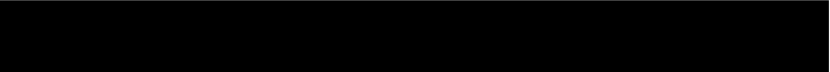
\includegraphics[width=1.2\paperwidth]{Logos/UCL page footer.png}
      }}
      

\thispagestyle{headings}
\maketitle
\FloatBarrier
\pagenumbering{roman}


\thispagestyle{empty}
\begin{figure}[H]
    \centering
    
\includegraphics[width=0.95\linewidth]{Screenshot 2025-04-01 at 16.30.45.png}
\end{figure}


\thispagestyle{empty}
\begin{abstract}
Quantum computing promises revolutionary advances across various fields, including cryptography, complex simulations, and optimisation problems. However, practical implementation faces substantial hurdles, many of which arise from challenges in quantum error correction (QEC), particularly the high resource overhead and gate complexity in fault-tolerant computations. Existing methods for optimising logical Clifford operations in stabiliser codes often suffer from computational inefficiency or limited scalability. To address this, this thesis introduces an algorithmic approach based on a theory by Dr. Mark Webster. Our goal is to reduce the complexity of logical Clifford operations by finding implementations that can be decomposed into SWAPs, single-qubit Cliffords, and as few two-qubit transvections as possible. The solution employs an evolutionary search framework, combining elitism, tournament selection, adaptive mutation, and parameter tuning to efficiently navigate the solution space. The methodology was rigorously tested on benchmark stabiliser codes such as [[5,1,3]] and [[7,1,3]], and applied to the topologically significant [[8,2,2]] Toric code to showcase its ability to discover previously undocumented logical Clifford gate implementations. Key achievements include an efficient constant-depth implementation of the logical S gate and relatively low-depth versions of H, CZ, and CNOT gates. Quantitative results show a high success rate of up to \(86\%\) for smaller codes \(n<7\). To the best of our knowledge, this is the first reported approach to identify logical Clifford operators for general [[n,k,d]] stabiliser codes, underscoring its potential for improving implementations in both familiar and unexplored codes. Future work could integrate machine learning to further improve adaptability and performance on larger, more complex quantum codes.


% \vspace{-10mm} %To remove added white space after
\end{abstract}





\tableofcontents

\thispagestyle{plain}
\listoffigures
\listoftables
%\lstlistoflistings
\listofalgorithms


%%%%%%%%%%%%%%%%%%%%%%%%%%%%%%%%%%%%%%%%%%%%%%%%%%%%%%%%%%%%%%%%%%%%%%%%%%%%%%%%
\chapter{Introduction and Background} \label{Chap2}
\pagenumbering{arabic}

\section{Introduction}
Quantum computing promises to solve otherwise unsolvable problems. More specifically, problems that would be practically impossible to solve on a classical computer. At the heart of quantum computing lies quantum mechanics, a theory fundamentally different from classical physics. While classical computers encode information in binary digits (bits) that take on definite states of either 0 or 1, quantum computers leverage quantum bits (qubits) which can exist in superpositions of both states simultaneously. This unique property allows quantum computers to explore multiple possibilities concurrently, providing exponential computational advantages for certain classes of problems. Moreover, quantum entanglement, another fundamental quantum phenomenon, enables powerful correlations between qubits that significantly enhance computational efficiency and information processing capabilities. These principles underlie quantum algorithms such as Shor's algorithm for integer factorisation \cite{365700} and Grover's algorithm for unstructured search \cite{10.1145/237814.237866}, each offering dramatic speed-ups over classical counterparts. Additionally, quantum computers are particularly adept at simulating complex quantum systems such as molecules, chemical reactions, or condensed matter phenomena which classical computers handle inefficiently due to exponential resource demands. 

The quantum states underlying these remarkable advantages are inherently fragile. Unlike classical bits, qubits maintain coherence the delicate quantum mechanical property essential for computation only under stringent environmental isolation. Even slight interactions with the external environment, such as thermal fluctuations, electromagnetic radiation, or unintended coupling with neighboring qubits, can quickly degrade quantum coherence. This phenomenon, known as decoherence, rapidly reduces the quantum state from a coherent superposition into a classical probabilistic mixture, thereby erasing quantum advantages and introducing significant errors into computations. Additionally, quantum gates operations used to manipulate quantum states are themselves imperfect. Gate operations introduce systematic errors due to inaccuracies in control signals, calibration imperfections, and hardware limitations, collectively diminishing computational reliability \cite{bultrini2020simplemitigationstrategysystematic}.

Besides improvements to hardware such as enhancing qubit quality, isolation from environmental noise, and precision control of quantum operations, addressing these significant challenges also requires fault-tolerant quantum error correction methods \cite{Calderbank_1996}. Fault tolerance broadly refers to the ability of a quantum computing system to detect, isolate, and correct errors without compromising quantum coherence or the integrity of quantum information \cite{cdi_askewsholts_vlebooks_9780511985249}. Achieving fault tolerance is critical because quantum errors cannot be eliminated entirely due to fundamental physical limitations. By employing carefully designed protocols and optimised quantum circuits, fault-tolerant quantum computing ensures computations can proceed reliably despite the inevitability of errors. Crucially, an essential element of fault-tolerant quantum computing is the efficient design and minimisation of quantum circuits. Minimising quantum circuits reduces exposure to environmental noise, lowers error rates \cite{yu2022analysiserrorpropagationquantum}, and improves overall computational accuracy and scalability.

The necessity to execute quantum algorithms efficiently with the fewest possible operations highlights the importance of circuit optimisation techniques. Efficient circuit implementations are vital to maintain coherence, minimise resource consumption, and maximise the practical utility of quantum computing hardware. Consequently, the central objective of this research is to design a search algorithm specifically tailored to identify the logical implementation of Clifford operations that uses the fewest possible number of two-qubit gates, namely transvections. By designing a metaheuristic search algorithm and selecting optimal logical operator implementations, this project seeks to provide a means to significantly reduce circuit complexity, lower error rates, and improve quantum computational efficiency. Ultimately, this contributes directly to the broader goal of realising robust, scalable, and fault-tolerant quantum computing technologies.

\section{Background}
\subsection{Quantum Error Correction}
As mentioned before, quantum systems are inherently fragile due to the numerous errors arising from interactions with the external environment. Unlike classical information bits, quantum bits (qubits) cannot be copied due to the no-cloning theorem \cite{Wootters1982ASQ}, nor can they be measured without causing the collapse of the quantum state. These constraints make classical redundancy-based error correction challenging to implement. Quantum error correction (QEC) circumvents these limitations by encoding logical quantum information into entangled states across multiple physical qubits, leveraging quantum entanglement and superposition to distribute the information of a single logical qubit. This encoding process protects logical qubits against errors, including bit flips, phase flips, and decoherence-induced errors.

The general structure of error correction is a two-step process: error detection and recovery \cite{cdi_askewsholts_vlebooks_9780511985249}. During error detection, the quantum state undergoes syndrome measurements that identify whether an error has occurred without directly observing the quantum information itself, thereby preserving coherence. The measured syndrome does not reveal the quantum information stored but rather indicates the specific type and location of errors within the encoded quantum state. In the recovery step, this information guides the application of corrective operations that reverse the detected errors, restoring the quantum state to its intended logical form. Through this careful combination of detection and corrective actions, QEC can help to maintain computational reliability and facilitate scalable, fault-tolerant quantum computing.

\begin{figure}[h]
    \centering
    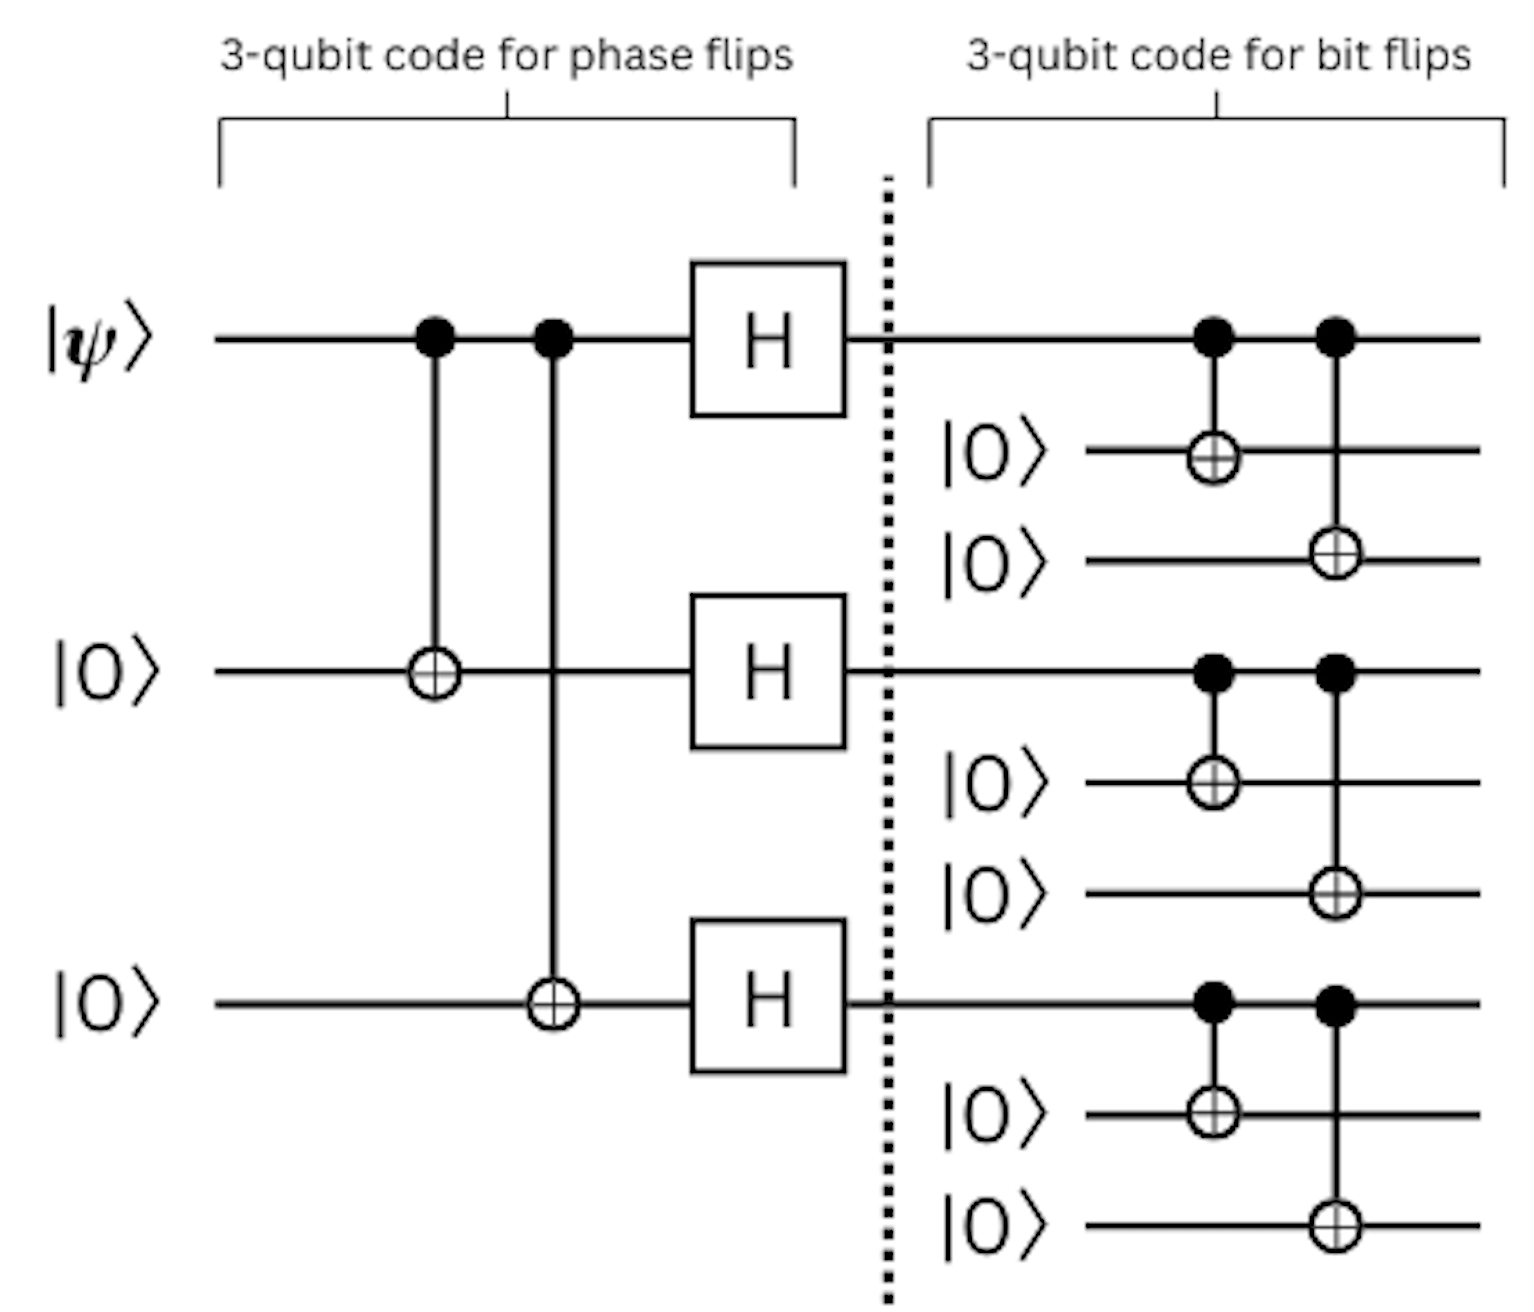
\includegraphics[width=0.5\linewidth]{Logos/Screenshot 2025-03-26 at 21.37.08.png}
    \caption{Circuit diagram of the [[9,1,3]] Shor Code}
    \label{fig:Shor Code Circuit}
\end{figure}

One famous example of an error correction code is the [[9,1,3]] Shor code \cite{PhysRevA.52.R2493} illustrated in Figure \ref{fig:Shor Code Circuit}. The Shor code encodes one logical qubit into nine physical qubits (see equation \ref{eq:logical states}) and is capable of detecting arbitrary two-qubit errors and correcting any single-qubit error. It achieves this by combining two simpler quantum codes: the 3-qubit bit-flip code and the 3-qubit phase-flip code. 

The bit-flip code protects against \(X\) errors, which flip the state of a qubit from |\(0\rangle\) to |\(1\rangle\) or vice versa. It works by encoding a logical qubit into three physical qubits as:

\begin{equation}
    |0_L\rangle=|000\rangle, \quad|1_L\rangle=|111\rangle
\end{equation}

A single bit-flip can be detected by checking parity between qubit pairs and corrected by flipping the erroneous qubit.

The phase-flip code works similarly in the Hadamard basis to protect against \(Z\) errors by detecting phase mismatches. It encodes the logical qubit as:

\begin{equation}
    |0_L\rangle=|+++\rangle, \quad|1_L\rangle=|---\rangle
\end{equation}

where,

\begin{equation}
    |\pm\rangle=\frac{1}{\sqrt{2}}(|0\rangle\pm|1\rangle
\end{equation}

The Shor code concatenates these two codes: it first encodes a logical qubit using the phase-flip code across three blocks, then applies the bit-flip code within each block of three qubits, resulting in the following encoded state:

\begin{equation}
\label{eq:logical states}
    |\psi\rangle = \alpha|0\rangle + \beta|1\rangle \rightarrow |\psi_L\rangle = \alpha|0_L\rangle + \beta|1_L\rangle
\end{equation}

where,

\begin{equation}
    |0_L\rangle=\frac{1}{\sqrt{8}}(|000\rangle+|111\rangle)\otimes(|000\rangle+|111\rangle)\otimes(|000\rangle+|111\rangle)
\end{equation}

and,

\begin{equation}
    |1_L\rangle=\frac{1}{\sqrt{8}}(|000\rangle-|111\rangle)\otimes(|000\rangle-|111\rangle)\otimes(|000\rangle-|111\rangle)
\end{equation}

The layered structure allows the Shor code to detect and correct any single-qubit error bit-flip, phase-flip, or both by measuring stabilisers that reflect parity and phase relationships without collapsing the encoded quantum information. This layered structure allows the Shor code to address both major types of quantum noise, making it a powerful demonstration of how quantum information can be preserved through entanglement and redundancy. Despite its conceptual simplicity, the Shor code captures many of the essential ideas behind more advanced quantum error-correcting codes used in practice today.

\subsection{Stabiliser Formalism}
Stabiliser codes are among the most widely used quantum error correction methods, built upon the mathematical framework of stabiliser formalism. In this approach, quantum states are described by sets of commuting Pauli operators, called stabilisers, which leave the encoded state invariant. Specifically, a unitary operator \(U\) stabilises a state |\(\psi\rangle\) if ,
\begin{equation}
    U|\psi\rangle=|\psi\rangle
\end{equation}
These stabilisers are typically expressed as tensor products of single qubit Pauli operators \(X, Y\), and \(Z\), which satisfy the relations, \(X^2=Y^2=Z^2=I\) and and specific rules outlined in Table \ref{tab:pauli relations}.

\begin{table}[h]
\label{}
\centering
\[
\begin{array}{c|ccc}
 & X & Y & Z \\
\hline
X & 0 & iZ & -iY \\
Y & -iZ & 0 & iX \\
Z & iY & -iX & 0 \\
\end{array}
\]
\caption{Relations of the Pauli operators (entry shows the value of the row times the column).}
\label{tab:pauli relations}
\end{table}

Set of equations defining the actions of \(X, Y\), and \(Z\).

\begin{equation}    
\label{eq:actions of pauli operators}
\begin{aligned}
X \ket{0} &= \ket{1}, & \quad X \ket{1} &= \ket{0} \\
Y \ket{0} &= i\ket{1}, & \quad Y \ket{1} &= -i\ket{0} \\
Z \ket{0} &= \ket{0}, & \quad Z \ket{1} &= -\ket{1}
\end{aligned}
\end{equation}

Using these properties we can demonstrate stabiliser formalism. As an example consider the Bell state,

\begin{equation}
    |\Phi^+\rangle = \frac{\ket{00}+\ket{11}}{\sqrt{2}}
\end{equation}

It is easy to verify that the Pauli operators \(Z_1Z_2\), \(X_1X_2\) and their product, \(-Y_1Y_2\), stabilise |\(\Phi^+\rangle\), since applying all three Pauli operators leaves the state unchanged. Together, these Pauli operators form the stabiliser group of |\(\Phi^+\rangle\), which consists of all operators under which the state remains invariant. An essential property of any stabiliser group is that all its members mutually commute, ensuring that they share a common set of eigenstates. The set of all such shared +1 eigenstates defines the code space, a subspace of the full Hilbert space in which the logical quantum information is encoded and protected. For single state stabiliser codes like |\(\Phi^+\rangle\), this code space is one-dimensional and uniquely determined by the stabiliser group.

Rather than listing the entire stabiliser group, it is often more efficient to describe the state using a stabiliser generator group, a minimal set of independent stabilisers whose combinations generate the full group. In the case of |\(\Phi^+\rangle\), the stabiliser generator group, denoted by \(\langle S\rangle\), is simply \(Z_1Z_2\) and \(X_1X_2\). It turns out that for many QEC codes, stabiliser formalism allows for a more compact and efficient way of representing states as opposed to the typical vector amplitude representation. In particular, quantum circuits composed entirely of Clifford gates such as CNOT, Hadamard, and phase gates are especially well suited to this framework, as these gates preserve the stabiliser structure under conjugation and allow for efficient classical simulation \cite{Aaronson_2004}.

Building on the utility of stabiliser generators, a convenient and compact way to represent them is through the check matrix (also known as the stabiliser tableau). This is a binary matrix of dimensions \(|\langle S \rangle | \times 2n\), where \(n\) is the number of qubits and \(|\langle S \rangle |\) is the number of stabiliser generators. Each row corresponds to one generator, with the first \(n\) columns encoding the presence of \(X\) operators on each qubit and the last \(n\) columns encoding the presence of \(Z\) operators. The presence of a \(Y\) operator is indicated by a 1 in both the \(X\) and \(Z\) components for that qubit. This binary representation greatly simplifies the manipulation and simulation of stabiliser codes, particularly for circuits composed of Clifford operations. It is important to note that the check matrix captures the structure of the generators up to a global phase, which has no effect on the error detecting or error correcting capabilities of the code \cite{webster2024engineeringquantumerrorcorrection}. Despite abstracting away these phases, the check matrix formalism maintains all the essential information needed for error detection and recovery, while remaining computationally efficient and scalable. As an example, the previously discussed \([[9,1,3]]\) Shor code encodes one logical qubit into nine physical qubits and protects against single-qubit errors through combined bit-flip and phase-flip correction, as reflected in its stabiliser generators below.

\begin{table}[h]
\centering
\begin{tabular}{c l}
\toprule
\textbf{Stabilisers } & \textbf{Operator (X, Z)} \\
\midrule
\(S_1\) & \( X_1 X_2 X_3 X_4 X_5 X_6 \) \\
\(S_2\) & \( X_4 X_5 X_6 X_7 X_8 X_9 \) \\
\(S_3\) & \( Z_1 Z_2 \) \\
\(S_4\) & \( Z_2 Z_3 \) \\
\(S_5\) & \( Z_4 Z_5 \) \\
\(S_6\) & \( Z_5 Z_6 \) \\
\(S_7\) & \( Z_7 Z_8 \) \\
\(S_8\) & \( Z_8 Z_9 \) \\
\bottomrule
\end{tabular}
\caption{Stabiliser Generators for the [[9,1,3]] Shor Code.}
\label{tab:shor code generators}
\end{table}

In check matrix form we can represent this code as,

\begin{equation}
\label{eq:shor code check matrix}
\begin{bmatrix}
1 & 1 & 1 & 1 & 1 & 1 & 0 & 0 & 0 \; &\; 0 & 0 & 0 & 0 & 0 & 0 & 0 & 0 & 0 \\
0 & 0 & 0 & 1 & 1 & 1 & 1 & 1 & 1 \; &\; 0 & 0 & 0 & 0 & 0 & 0 & 0 & 0 & 0 \\
0 & 0 & 0 & 0 & 0 & 0 & 0 & 0 & 0 \; &\; 1 & 1 & 0 & 0 & 0 & 0 & 0 & 0 & 0 \\
0 & 0 & 0 & 0 & 0 & 0 & 0 & 0 & 0 \; &\; 0 & 1 & 1 & 0 & 0 & 0 & 0 & 0 & 0 \\
0 & 0 & 0 & 0 & 0 & 0 & 0 & 0 & 0 \; &\; 0 & 0 & 0 & 1 & 1 & 0 & 0 & 0 & 0 \\
0 & 0 & 0 & 0 & 0 & 0 & 0 & 0 & 0 \; &\; 0 & 0 & 0 & 0 & 1 & 1 & 0 & 0 & 0 \\
0 & 0 & 0 & 0 & 0 & 0 & 0 & 0 & 0 \; &\; 0 & 0 & 0 & 0 & 0 & 0 & 1 & 1 & 0 \\
0 & 0 & 0 & 0 & 0 & 0 & 0 & 0 & 0 \; &\; 0 & 0 & 0 & 0 & 0 & 0 & 0 & 1 & 1 \\
\end{bmatrix}
\end{equation}

Expressing a code in check matrix form enables efficient manipulation using binary linear algebra over \(\mathbb{F}_2\) \cite{webster2024engineeringquantumerrorcorrection}. Pauli operators (up to global phase) can be treated as binary vectors, allowing operations like Gaussian elimination to identify independent stabiliser generators. Row additions correspond to multiplying stabilisers, while column operations reflect Clifford conjugation or qubit relabelling. These transformations preserve the code structure, making the check matrix a compact and powerful tool for analysing and evolving stabiliser codes.

\subsection{Logical Operators}
Building on the structure defined by the stabiliser group, a complete description of a stabiliser code also requires specifying the logical operators. While the stabiliser group defines the code space as the simultaneous +1 eigenspace of its generators, logical operators act within this space to manipulate the encoded quantum information. These are Pauli operators that commute with all elements of the stabiliser group ensuring they preserve the code space but are not themselves part of the stabiliser group. This distinction allows them to act non-trivially on the encoded logical qubits. Importantly, because the Pauli group can be represented as a vector space over \( \mathbb{F}_2 \), logical operators can also be expressed and manipulated within the check matrix framework. Identifying logical operators thus becomes an extension of the same algebraic techniques used for analysing stabilisers. These operators are essential for performing computation on encoded qubits, enabling operations such as logical \(X\), \(Z\), or even Clifford gates to be applied directly to encoded data without requiring decoding.

As an example we will look at the [[9,1,3]] code shown in Table \ref{tab:shor code generators}. Here I will simply provide the logical operators for \(X\) and \(Z\), denoted as \(\overline{X}\) and \(\overline{Z}\), to demonstrate their action on the stabiliser group as the method for their construction has been well documented (see papers \cite{webster2024engineeringquantumerrorcorrection} \cite{cdi_askewsholts_vlebooks_9780511985249} for full detail on the construction of Logical \(X\) and \(Z\) from check matrix). The logical \(X\) and \(Z\) are defined as

\begin{equation}
    \overline{X}=Z_1Z_4Z_7, \quad \overline{Z}=X_1X_2X_3
\end{equation}

These operators are not part of the stabiliser group, as they are neither among the generators nor expressible as products of them. However, they commute with all elements of the stabiliser group, ensuring they preserve the code space, and they act non-trivially within it. Like their single-qubit Pauli analogues \(\overline{X}\) and \(\overline{Z}\), consistent with the canonical Pauli relations (see Table \ref{tab:pauli relations}). Moreover, when applied to the encoded logical states of the Shor code (see Equation \ref{eq:logical states}), these logical operators reproduce the standard Pauli actions (see Equation \ref{eq:actions of pauli operators}). These properties confirm that \(\overline{X}\) and \(\overline{Z}\) faithfully implement logical operations on the encoded qubit, just as \(X\) and \(Z\) do in the unencoded single-qubit case.

\subsection{The Clifford Group}
In the context of stabiliser codes, applying arbitrary unitary operations to encoded quantum states can pose a serious problem. Ideally, operations performed on encoded qubits should preserve the structure of the stabiliser group, ensuring that the resulting state remains within the protected code space. However, generic unitary gates can map Pauli operators to non-Pauli operators under conjugation, thereby disrupting the stabiliser structure and potentially introducing undetectable errors. This breaks the assumptions of the stabiliser formalism, which relies on all stabilisers being elements of the Pauli group.

To address this issue, quantum error correction restricts operations to a special subset of unitary gates known as the Clifford group. The Clifford group is defined as the set of unitaries, \(U\), that map Pauli operators, \(M\), to other Pauli operators, \(M'\), under conjugation \cite{gottesman2016surviving} i.e.

\begin{equation}
    UMU^{\dagger}=M'
\end{equation}

This property guarantees that the transformed stabiliser group remains entirely within the Pauli group, preserving error detectability and compatibility with syndrome measurement. The Clifford group includes gates such as the Hadamard (H), Phase (S), and controlled-NOT (CNOT), all of which are foundational to quantum error correction and fault-tolerant quantum computation, however they are not universal for quantum computation.

A key feature of the Clifford group is its homomorphism to the binary symplectic group, meaning that Clifford gates can be represented as binary symplectic matrices. A binary symplectic matrix is a \(2n\times2n\) matrix over \(\mathbb{F}_2 \) that preserves the symplectic inner product \cite{rengaswamy2018synthesis}, a bilinear form that encodes the commutation relationships of Pauli operators. Specifically, a matrix \(M\) is symplectic if it satisfies:

\begin{equation}
\label{eq:symplectic matric property}
    M^T\Omega M=\Omega,
\end{equation}
where,
\begin{equation}
    \Omega = 
    \begin{bmatrix}
    0 & I_n \\
    I_n & 0 \\
    \end{bmatrix}
\end{equation}

This condition ensures that conjugation by a Clifford gate preserves the commutation and anti-commutation structure of Pauli operators. The symplectic representation enables the use of efficient classical algorithms to simulate and manipulate Clifford operations without requiring full complex-valued unitary matrices. For instance, each Clifford gate can be mapped to a symplectic matrix that reflects how it transforms Pauli operators under conjugation. The Hadamard gate, for example, swaps \(X\) and \(Z\) under conjugation, and is represented by the symplectic matrix:

\begin{equation}
H=
\begin{bmatrix}
    0 & 1 \\
    1 & 0 \\
\end{bmatrix}
,
\end{equation}

where the first row corresponds to where \(X\) is mapped to,  and the second row corresponds to where \(Z\) is mapped to. Specifically, under conjugation by the Hadamard gate, \(X\rightarrow Z\) and \(Z\rightarrow X\). This action is reflected in the matrix, the \(X\) component (first column) is swapped with the \(Z\) component (second column). We can also easily verify H upholds Equation \ref{eq:symplectic matric property}, confirming that it preserves the symplectic inner product and thus maintains the commutation relations between Pauli operators under conjugation.

Another powerful feature of the stabiliser formalism is its ability to track the evolution of stabiliser codes under Clifford operations using the tableau representation(see paper Engineering quantum error correction codes using
evolutionary algorithms \cite{webster2024engineeringquantumerrorcorrection} for complete description):

\begin{equation}
    \tau=
    \begin{bmatrix}
        S_x \\
        S_z \\
        L_z \\
        R_x \\
        R_z \\
        L_x
    \end{bmatrix},
\end{equation}

where,

\begin{equation}
    \begin{bmatrix}
        R_x\\
        R_z
    \end{bmatrix}
    =
    \begin{bmatrix}
        0&0&0&I&0&0\\
        0&I&0&0&0&0
    \end{bmatrix}
\end{equation}

In this structure, \(S_x\) and \(S_z\) represent the \(X\) and \(Z\) components of the stabiliser generators that define the code space. The rows \(L_x\) and \(L_z\) correspond to the logical Pauli operators (previously denoted as \(\overline{X}\) and \(\overline{Z}\)) that act non-trivially on the encoded qubits while preserving the stabiliser group. The remaining rows, \(R_x\) and \(R_z\), are known as the destabilisers, which form part of a full operator basis and are essential for decoding and syndrome analysis. Together, these blocks of the tableau encode the full algebraic structure of the stabiliser code and support efficient classical simulation \cite{Aaronson_2004}, encoding transformations, and the implementation of logical operations within the Clifford framework.
The tableau format encodes the stabiliser generators, logical operators, and destabilisers as binary symplectic matrices, enabling compact and efficient simulation of quantum error correcting codes. This structure preserves the symplectic inner product and thus the commutation relationships among Pauli operators, even as Clifford operations transform them.

The tableau representation is particularly useful because it not only compactly captures the structure of stabiliser codes but also acts as an encoding operator. It maps an initial quantum state, consisting of \(k\) logical qubits and \(n-k\) ancillary qubits, into an encoded state within the stabilised code space of \(n\) physical qubits. This transformation is expressed by the following mapping:

\begin{equation}
\begin{large}
\begin{tikzcd}
\mathcal{H}_2^{n-k} \otimes \mathcal{H}_2^k \arrow[r, "\mathcal{\tau}"]  &
\mathcal{H}_2^n
\end{tikzcd}
\end{large}
\end{equation}

Here, \(\mathcal{H}_2^k\)  represents the Hilbert space of the \(k\) logical qubits containing the input quantum information, while \(\mathcal{H}_2^{n-k} \) represents the ancillary qubits initialised in known basis states (typically \(|0\rangle\)). Specifically, given a Clifford operator associated with a binary symplectic matrix \(\tau\), the tableau allows us to construct an encoding circuit that implements the transformation |\(\psi\rangle \rightarrow |\overline{\psi}\rangle\), embedding logical qubits into a protected subspace.

Clifford operations can also be composed using (symplectic) transvections, a type of symplectic transformation that acts minimally on the qubit register and is particularly useful for reducing the number of two-qubit gates. Since two-qubit gates are typically more error-prone than single-qubit gates due to the complex interactions and control precision required for entangling operations between qubits \cite{maldonado2022error}, minimising their use is crucial for building robust and fault-tolerant quantum circuits. Expressing Clifford circuits as sequences of transvections provides an efficient way to reduce circuit depth and control error propagation.

A symplectic transvection is a special kind of operator 

\begin{equation}
\label{eq:transvection definition}
    T_v=I+\Omega v^Tv
\end{equation}

where \(v\in \mathbb{F}_2^{2n} \) \cite{volanto2023minimizing}. In the Clifford domain, they correspond to operations that conjugate Pauli operators in a structured way and can be interpreted as square roots of Pauli matrices. Importantly, any Clifford operator can be decomposed into a product of at most \(2n\) such transvections, meaning they form a universal generating set for the symplectic group. Specific Clifford gates also have simple transvection decompositions, for example a CNOT gate can be written as a product of three transvections:

\begin{equation}
    CNOT_{i,j}=T_{[e_j,0]}T_{[e_j,e_i]}T_{[0,e_i]}
\end{equation}

This decomposition framework makes transvections a powerful tool for designing low-depth Clifford circuits with minimal two-qubit gate usage, as explored in \cite{volanto2023minimizing}.


\section{Project Aim}
While not universal for quantum computation, the Clifford group underpins most quantum error correction schemes by enabling fast, fault-tolerant logical gate implementations that preserve stabiliser structures. Any logical Clifford operator can be decomposed into transvections, SWAPs, and single-qubit Cliffords, with transvections, requiring error-prone two-qubit gates, being the most costly \cite{volanto2023minimizing}. This project develops a search algorithm to minimise transvections in such decompositions, thereby enhancing the efficiency and fault-tolerance of stabiliser code implementations for scalable quantum computing.
%%%%%%%%%%%%%%%%%%%%%%%%%%%%%%%%%%%%%%%%%%%%%%%%%%%%%%%%%%%%%%%%%%%%%%%%%%%%%%%%
\chapter{Methodology} \label{Chap3}

\section{Theorem behind the Search Algorithm}

\subsection{Producing All Logical Cliffords}
The underlying theorem behind the search algorithm was found by my supervisor Dr. Mark Webster (paper under development). The theorem can be described as follows:

\begin{theorem}
    Let \(\tau\) be the symplectic matrix (tableau) of the encoding operator of an \([[n,k]]\) stabiliser code and let $U$ be a Clifford unitary on \(k\) qubits. The logical Clifford operators with action \(U\) are of the form:
    \begin{equation}
    \label{eq:Generation of Logical operator}
        \bar{U}:=\tau^{-1}\left(\left( I\otimes U\right)U_C U_A\right)\tau
    \end{equation}
    where \(U_A, U_C\) have symplectic representations of the following form:
    \begin{equation}
        U_A := \left[\begin{array}{cc|cc}I&0&0&0\\0&I&0&0\\\hline A_1&A_2^T&I&0\\A_2&0&0&I\end{array}\right]
    \end{equation}
    \begin{equation}
        U_C := \left[\begin{array}{cc|cc}C_1&0&0&0\\C_2&I&0&0\\\hline 0&0&C_1^{-T}&C_1^{-T}C_2^T\\0&0&0&I\end{array}\right]
    \end{equation}
    
    Note that symplectic matrices act on Paulis by right matrix multiplication, so order of operations is reversed. In the above forms, \(r:=n-k\),  \(A_1\) is a symmetric \(r\times r\) matrix, \(C_1\) is an invertible \(r\times r\) matrix, \(A_2,C_2\) are arbitrary \(k\times r\) matrices and  \(C_1^{-T} := \left(C_1^{-1}\right)^T\).
\end{theorem}

This theorem states that given a unitary Clifford operator, \(U\), and the encoding operator, \(\tau\),  we can create all Logical Cliffords, \(\bar{U}\), with the desired action \(U\), by considering all possible forms of \(U_A\) and \(U_C\). The figure below provides an intuitive visualisation of Equation \ref{eq:Generation of Logical operator}.We can interpret the logical operation \(\bar{U}\) as a three-step process: first, the encoded quantum state is decoded by applying the inverse of the encoding operation, \(\tau^{-1}\), then, the desired single-qubit Clifford operation \(U\) is applied to the logical subspace; and finally, the state is re-encoded using \(\tau\), mapping it back into the protected code space. This sequence effectively implements the logical Clifford \(\bar{U}\) on the encoded state by conjugating the logical action through the encoding circuit.

\begin{figure}[h]
    \centering
    \begin{large}
    \begin{tikzcd}
    \mathcal{H}_2^{n-k} \otimes \mathcal{H}_2^k \arrow[r, "\mathcal{\tau}"] \arrow[d, " (I \otimes U)\, U_C\, U_A"'] &
    \mathcal{H}_2^n \arrow[d, "\overline{U}"] \\
    \mathcal{H}_2^{n-k} \otimes \mathcal{H}_2^k \arrow[r, "\mathcal{\tau}"] &
    \mathcal{H}_2^n
    \end{tikzcd}
    \end{large}
    \caption{Hilbert space diagram for generating all logical Cliffords}
    \label{fig:Hilbert space diagram}
\end{figure}

An important corollary in the synthesis of logical Clifford operators is the count of distinct Clifford operators that implement a given logical action \(U\), up to signs and stabiliser equivalence (i.e., modulo Pauli operators). The total number of such implementations, \(N\), is given by,

\begin{equation}
\label{eq:number of possible logical cliffords}
   N=2^{2rk + r(r+1)/2}\prod_{0 \le i \le r-1}(2^r - 2^i)
\end{equation}

where \(r=n-k\) is the number of stabiliser generators. This expression arises from the number of valid choices for the matrices \(A_1,A_2,C_1,\) and \(C_2\) that define different Clifford encodings with the same logical effect. Specifically, \(A_1\) is any symmetric \(r\times r\) binary matrix, contributing \(2^{r(r+1)/2}\) possibilities, \(A_2\) and \(C_2\) are arbitrary \(r\times k\) binary matrices, each contributing \(2^{rk}\), and \(C_1\) is any invertible \(r\times r\) binary matrix, with \(\prod_{0 \le i \le r-1}(2^r - 2^i)\) valid choices. The resulting product accounts for the total number of distinct tableau encodings realising the same logical Clifford. 

Given the exponential number of possible logical Clifford implementations described by Equation \ref{eq:number of possible logical cliffords}, an exhaustive search over all valid combinations of \(A_1,A_2,C_1,\) and \(C_2\) becomes computationally infeasible for even modest values of \(n\) and \(k\) To overcome this, we have developed a search algorithm that leverages metaheuristic techniques to efficiently explore the vast solution space and identify logical Clifford implementations that minimise the number of two-qubit transvections. By focusing on solutions with the lowest entangling gate count, the algorithm finds not only optimal decompositions using two-qubit transvections, SWAPs, and single-qubit Clifford gates, but also does so with significantly reduced computational overhead compared to brute-force methods. The exponential reduction in time provided by using metaheuristic techniques is particularly valuable as there exist hundreds of stabiliser codes, each requiring its own distinct set of logical operators. The impracticality of brute-force synthesis across all codes makes scalable, optimised search strategies a crucial step toward practical fault-tolerant quantum circuit design.

\subsection{Decomposition of Logical Cliffords into SWAPs, 2-Qubit Transvections and Single-Qubit Cliffords}

In this section, we briefly mention the method used to decompose logical Clifford operators. The decomposition approach was developed by Kalle Volanto in his thesis Minimising the Number of Two-qubit Gates in Clifford Circuits \cite{volanto2023minimizing}, where a complete and detailed description of the method can be found. My supervisor, Mark, has implemented this decomposition in Python, allowing us to apply it directly to logical Cliffords. This is particularly important for our purposes, as it enables us to score the logical Cliffords based on the number of two-qubit transvections required. (see Appendix \ref{Appendix B} for more details)

\section{Algorithm Design}

\subsection{Overview of the Framework}
Given that we can decompose logical Cliffords into SWAPs,  2-Qubit Transvections and Single-Qubit Cliffords. The central goal of the algorithm is to identify the matrices \(U_A\) and \(U_C\) that construct a logical Clifford operator corresponding to a desired logical action, while minimising the number of two-qubit transvections required in its decomposition. This is achieved by exploiting the structure provided by the logical Clifford generation theorem (see Equation \ref{eq:Generation of Logical operator}), which allows all valid logical implementations to be expressed in terms of a parameterised family of symplectic matrices determined by the binary matrices 
\(A_1,A_2,C_1,\) and \(C_2\) .

The algorithm adopts a metaheuristic search strategy, inspired by evolutionary algorithms \cite{luke2009essentials}. It operates over a large, high-dimensional discrete space defined by candidate encodings of the matrices 
\(U_A\) and \(U_C\), which jointly determine the operator \((I \otimes U)\, U_C\, U_A\) in the logical construction. The algorithm begins by generating a large, random initial population of candidate \((U_C,U_A)\) pairs from the \(GL_2\) group. Each candidate is evaluated using a cost function that returns a score vector, where each entry corresponds to the number of two-qubit transvections involving a particular qubit, rather than a single total count. This scoring approach is advantageous because optimal decompositions tend to exhibit a more balanced distribution of transvections across qubits, as opposed to concentrating entangling operations on a small subset. In addition to this, finding solutions with a larger distribution of transvections across qubits are beneficial as concentrating two-qubit transvections on a limited subset of qubits can lead to increased local error rates and potential circuit bottlenecks.

A generational process is then used to iteratively refine the population. In each generation, a mixture of elitism (retaining the best performing candidates) and tournament selection (probabilistic selection based on performance) is used to choose individuals for reproduction. These selected candidates are mutated to introduce variation in the population, promoting exploration of the solution space. Two types of mutation operations are employed. The first involves performing row operations on the matrix \(C_1\), specifically adding one row to another modulo 2. This operation is well-suited to the structure of \(C_1\), as it preserves its invertibility, a necessary condition since \(C_1\) must remain an invertible \(r\times r\) matrix, and allows the algorithm to traverse the full space of invertible binary matrices \cite{gregor2024generatinginvertiblematricesrow}. The second type of mutation consists of applying arbitrary bit-flips to entries in a combined matrix containing \(A\) and \(C_2\). This is justified by the fact that both \(A_2\) and \(C_2\) are unconstrained binary matrices and can therefore be freely modified without violating structural requirements. For the symmetric matrix \(A_1\), its symmetry is maintained by restricting bit-flips to one side of the diagonal and reflecting the change across the diagonal, ensuring the matrix remains symmetric post-mutation.

These carefully designed mutations enable the algorithm to explore a broad and valid subset of the solution space efficiently, while ensuring that all algebraic constraints of the decomposition framework are respected. After mutation, the new population is re-evaluated, and the optimisation loop continues over multiple generations, gradually converging toward decompositions that minimise the number of two-qubit transvections.

Incorporating an adaptive mutation mechanism into the algorithm is crucial for addressing stagnation, which often arises when the search process becomes trapped in local minima. By detecting when improvements plateau, the algorithm can dynamically increase mutation strength, thereby enhancing exploration capabilities to escape these local optima and continue progressing toward high-quality solutions. This balance between exploration and exploitation is fundamental in evolutionary algorithms to maintain search efficacy across complex fitness landscapes.

To further enhance the robustness and search coverage of the algorithm, multiple independent populations are run in parallel. In our case we were able to simulate a maximum of 8 populations in parallel using multi-pool processing. Each process executes its own instance of the optimisation loop with a different random seed. This simple parallelisation strategy helps simulate a multi-start search without inter-process communication, improving the likelihood of finding globally optimal or near-optimal decompositions. This approach not only accelerates the discovery of promising regions in the search space but also reduces the risk of all search paths converging prematurely on local minima. Much like adaptive mutation, parallel independent populations provide an effective mechanism for diversifying the search trajectory, helping to ensure that global or near-global solutions are more likely to be found.

By combining efficient candidate generation, transvection-aware cost evaluation, and robust search dynamics, this framework provides a scalable and effective method for synthesising low-depth logical Clifford operators tailored to a given stabiliser code. The full procedure is outlined in Algorithm~\ref{alg:logical_clifford_construction}, which summarises the key steps of the search and optimisation process, from population initialisation through mutation, evaluation, and convergence. 

The pseudo code for the Algorithm is provided below. (See Appendix \ref{Appendix A} for sorce code)

\begin{algorithm}[H]
\caption{Algorithm for Optimal Logical Clifford Construction}
\label{alg:logical_clifford_construction}
\begin{algorithmic}[1]
\Require Encoding tableau \(\tau\), target Clifford \(U\)
\Ensure Optimal logical Clifford implementation \(\bar{U}\)
\State Compute inverse tableau \(\tau^{-1}\), set \(n, k, r = n-k\)
\State Initialise parameters, e.g population sise, number generations, ..., etc
\Statex
\State Randomly generate initial population of \((U_C, U_A)\) candidates
\State Create \(\bar{U}\) from Equation \ref{eq:Generation of Logical operator} using \(U,(U_A,U_C),\tau\), and \(\tau^{-1}\)
\State Decompose \(\bar{U}\) into 2-qubit transvections, SWAPS, and single qubit Cliffords 
\State Evaluate initial scores based on gate count on each qubit 
\State Store best candidate and score
\Statex
\For{each generation \(g\)}
    \State Select the top x (\(U_C,U_C\)) candidates by score (elite group)
    \State Select y others using tournament selection
    \Statex \hspace{1.5em} \(\rightarrow \) Randomly partition population into \(y\) groups (tournaments)
    \Statex \hspace{1.5em} \(\rightarrow \) In each group, evaluate scores of candidates
    \Statex \hspace{1.5em} \(\rightarrow \) Select the best-performing candidate from each group (winner)
    \State Combine elite group and tournament winners
    \Statex
    \State Mutate each candidate \(\lambda\) times to generate next generation
    \Statex
    \State Evaluate new population scores using steps 4-6
    \Statex
    \If{any candidate improves the best score}
        \State Update best score and reset stagnation counters
    \Else
        \State Increment stall and fertility counters
    \EndIf
    \If{stagnation exceeds threshold}
        \State Increase mutation strength to escape local minima
    \EndIf
    \If{transvection count = 0 (perfect solution found)}
        \State \textbf{break}
    \EndIf
\EndFor
\State \Return best score, best candidate
\end{algorithmic}
\end{algorithm}

\subsection{Parameter Selection and Tuning}
The performance and effectiveness of the algorithm are heavily influenced by the choice of several key parameters, including population size, number of mutations, mutation strength, elite fraction, tournament size, and the number of generations. Careful tuning of these parameters is essential to strike the right balance between exploration and exploitation, maximise convergence speed, and ensure that high-quality solutions are reliably found. To guide this selection process, a combination of empirical experimentation and theoretical intuition was employed.

Parameter tuning was carried out through a series of controlled small-scale tests on the \([[5,1,3]]\) and \([[7,1,3]]\) stabiliser codes to find zero 2-qubit transvection implementations of Logical \(H\), both of which have well-understood, constant-depth logical Clifford decompositions. For these codes we define the algorithms success by wether or not it is able to find an implementation of the logical Clifford with zero 2-qubit transvections. (Note: the success rate is for an individual population as opposed to looking at multiple populations in parallel). These benchmark codes provided a reliable foundation for evaluating algorithm performance. To ensure consistency and isolate the effect of individual parameters, each test was conducted using a fixed set of control parameters: a tournament size of 8, an elite fraction of 0.3, and no adaptive mutation. These values served as a baseline against which the impact of parameter variations could be measured.

Given the stochastic nature of metaheuristic algorithms, a fixed global random seed was used across all runs to ensure reproducibility and enable direct comparisons between different configurations under identical initial conditions. Success was defined as achieving a score of zero, meaning that the resulting logical Clifford decomposition required no two-qubit transvections, the most expensive operations in terms of error rate and circuit depth. In the following subsections, we examine the parameters to which the algorithm is most sensitive, supported by both experimental data and theoretical insights.

The first parameter we examine is the tournament size. Selecting an appropriate tournament size is especially important when considering how the algorithm should scale for larger stabiliser codes. We found that a reliable way to scale tournament size is by first considering the number of offspring each individual produces, denoted by \(\lambda\). The value of \(\lambda\) is designed to scale with the number of possible mutations an individual can undergo. As the code size increases, the mutation space grows rapidly, almost exponentially in practice. For instance, the \([[5,1,3]]\) code has 36 possible mutations, while the \([[7,1,3]]\) and \([[9,1,3]]\) codes have 78 and 136, respectively.

To maintain a healthy balance between exploitative (intensifying search around good solutions) and explorative (diversifying the search space) behaviour, we define \(\lambda\) as a fraction of the total number of mutation possibilities, specifically \((total\space possible\space mutations)/(n-1)\), which scales naturally with the number of qubits \(n\). Once \(\lambda\) is set, the tournament size can then be chosen to scale accordingly, ensuring that selection pressure remains balanced as the code scales. This adaptive approach helps maintain consistent algorithmic performance across a wide range of code sizes.

\begin{figure}[h]
    \centering
    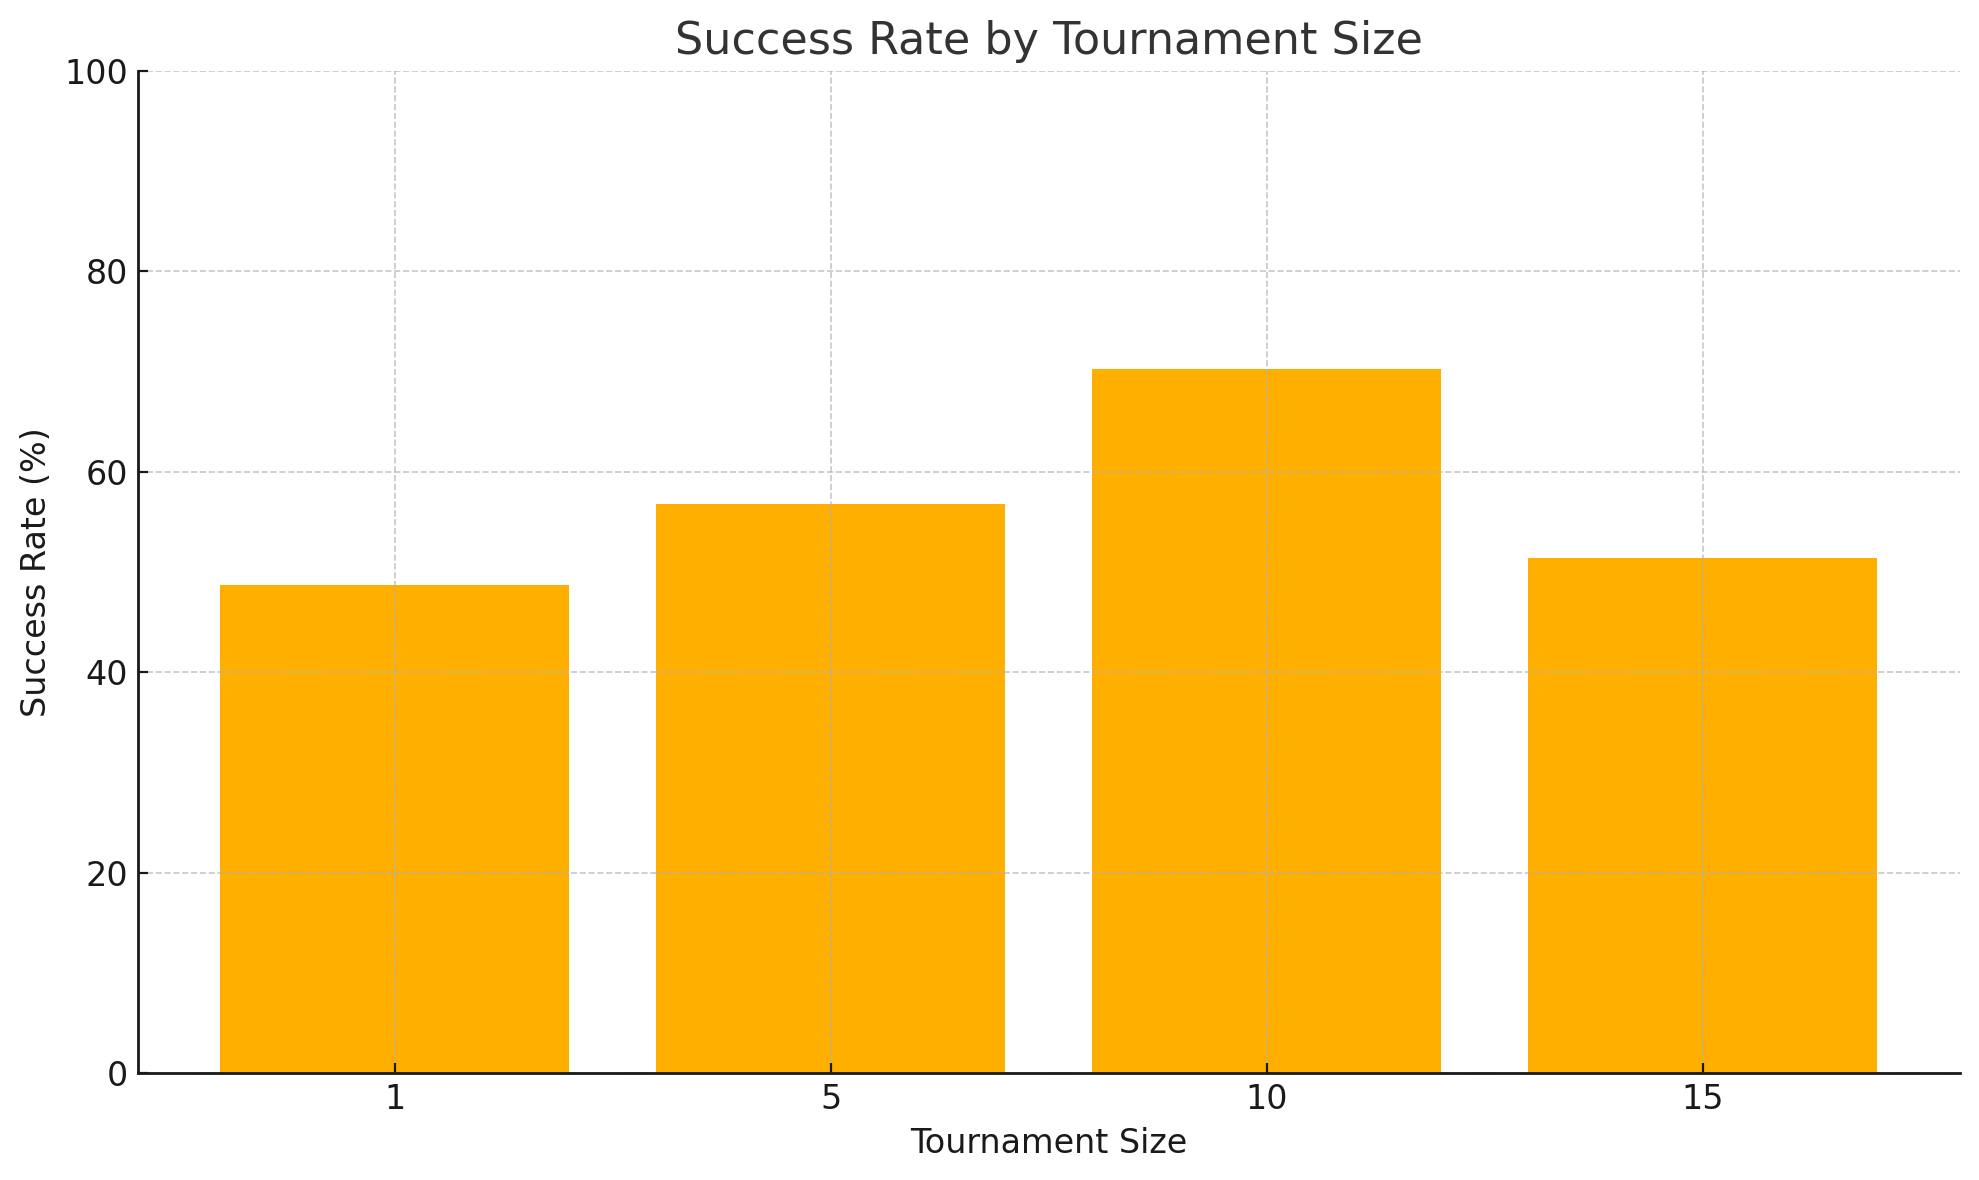
\includegraphics[width=1\linewidth]{Logos/output-2.png}
    \caption{Logical \(H\) Success rate on [[5,1,3]] code against tournament size. Number of runs = 38, elite fraction = 0.3.}
    \label{fig: tournament size chart}
\end{figure}

As shown in Figure \ref{fig: tournament size chart}, a tournament size of 10 yields the highest success rate of \(70.3\%\). This value coincides with a 1:1 ratio between \(\lambda\) and the tournament size, supporting the intuition that matching selection pressure to mutation scope leads to more effective search dynamics. Tournament sizes smaller than \(\lambda\) tend to reduce selection pressure, allowing weaker candidates to propagate and potentially slowing convergence. Conversely, larger tournament sizes increase selection pressure too aggressively, risking premature convergence to suboptimal solutions. These results affirm that scaling tournament size in proportion to \(\lambda\) provides a consistent and effective selection mechanism.

Another parameter to which the algorithm's success rate showed strong sensitivity is the elite fraction, which controls the proportion of candidates preserved from the previous generation through elitism. In this context, elites are defined as the individuals with the lowest number of two-qubit transvections, as measured by their score vectors. Adjusting the elite fraction directly influences the balance between exploitation, refining high-performing regions of the search space, and exploration, encouraging diversity and avoiding premature convergence.

A higher elite fraction places greater emphasis on preserving top candidates, which can accelerate convergence but also risks trapping the algorithm in local minima due to reduced variation. On the other hand, a lower elite fraction introduces more stochasticity through mechanisms like tournament selection, helping the algorithm explore new regions of the search space at the cost of slower convergence. 

\begin{figure}[h]
    \centering
    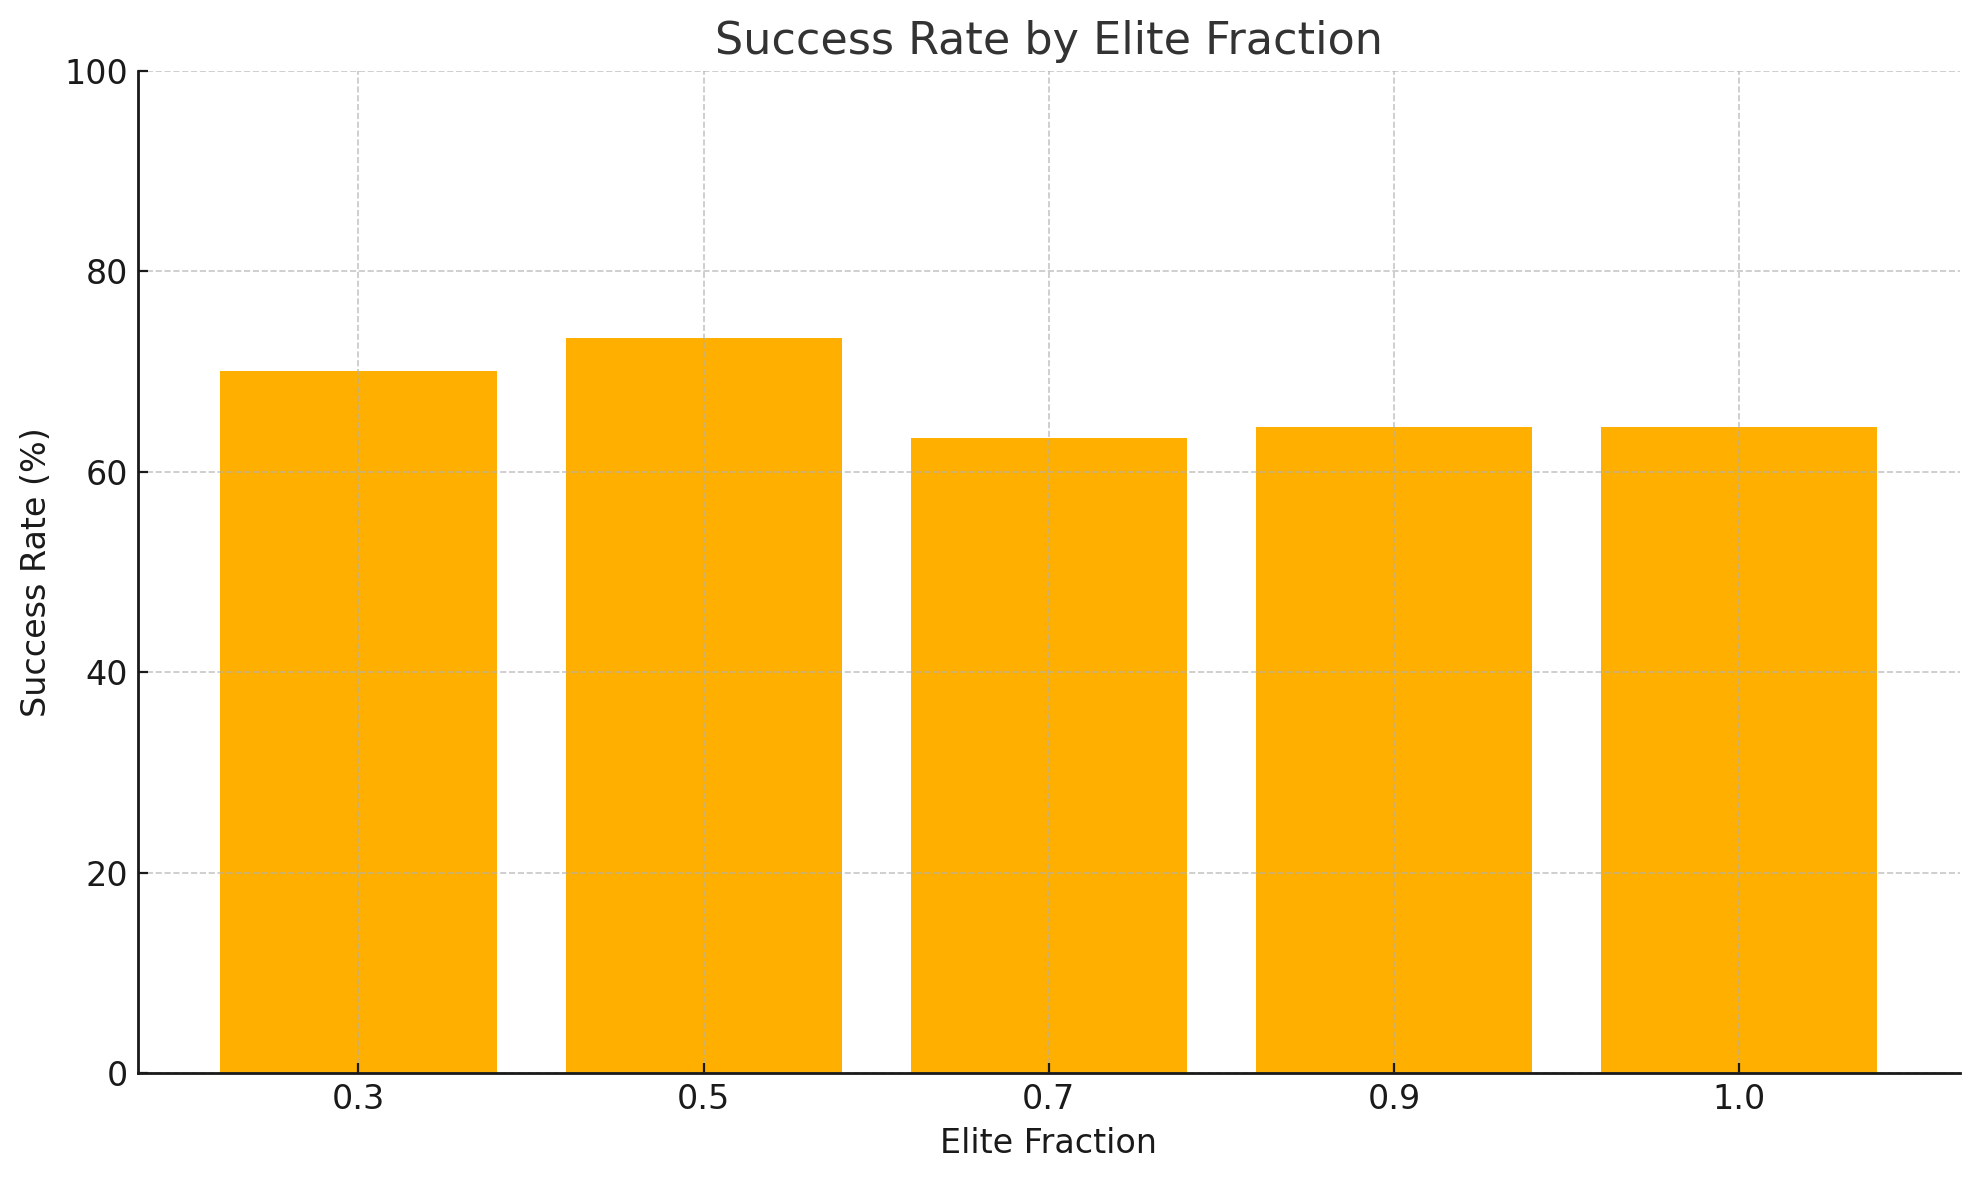
\includegraphics[width=1\linewidth]{Logos/output-3.png}
    \caption{Logical \(H\) Success rate on [[5,1,3]] code against elite fraction. Number of runs = 90, tournament size=8.}
    \label{fig: Elite fraction chart}
\end{figure}

As shown in Figure~\ref{fig: Elite fraction chart}, the highest success rate is achieved with an elite fraction of 0.5, reaching \(73.3\%\). This result supports the intuition that a balanced elitism strategy is most effective, preserving enough high-quality candidates to drive convergence, while still allowing sufficient diversity for the algorithm to escape local optima and generalise across different problem instances.

The final parameter we examine is the adaptive mutation mechanism, which plays a critical role in helping the algorithm escape local minima during the optimisation process. Several factors influence its design and effectiveness, including when to activate stronger mutations, how intense those mutations should be, and how frequently they are allowed to occur.

Our implementation uses a binary adaptive mutation strategy, alternating between two levels of mutation intensity: a fine-tuning mutation, where a single row operation or bit-flip is applied, and a strong mutation, where multiple such operations are performed on a single offspring. The central idea is that, when the population's performance stagnates, i.e., when no improvement is observed in the best candidate for several consecutive generations, it likely indicates that the search has become trapped in a local minimum. In these cases, strong mutation is temporarily activated to introduce more disruptive variation into the population, helping it escape the local basin of attraction and explore new regions of the search space.

\begin{figure}[h]
    \centering
    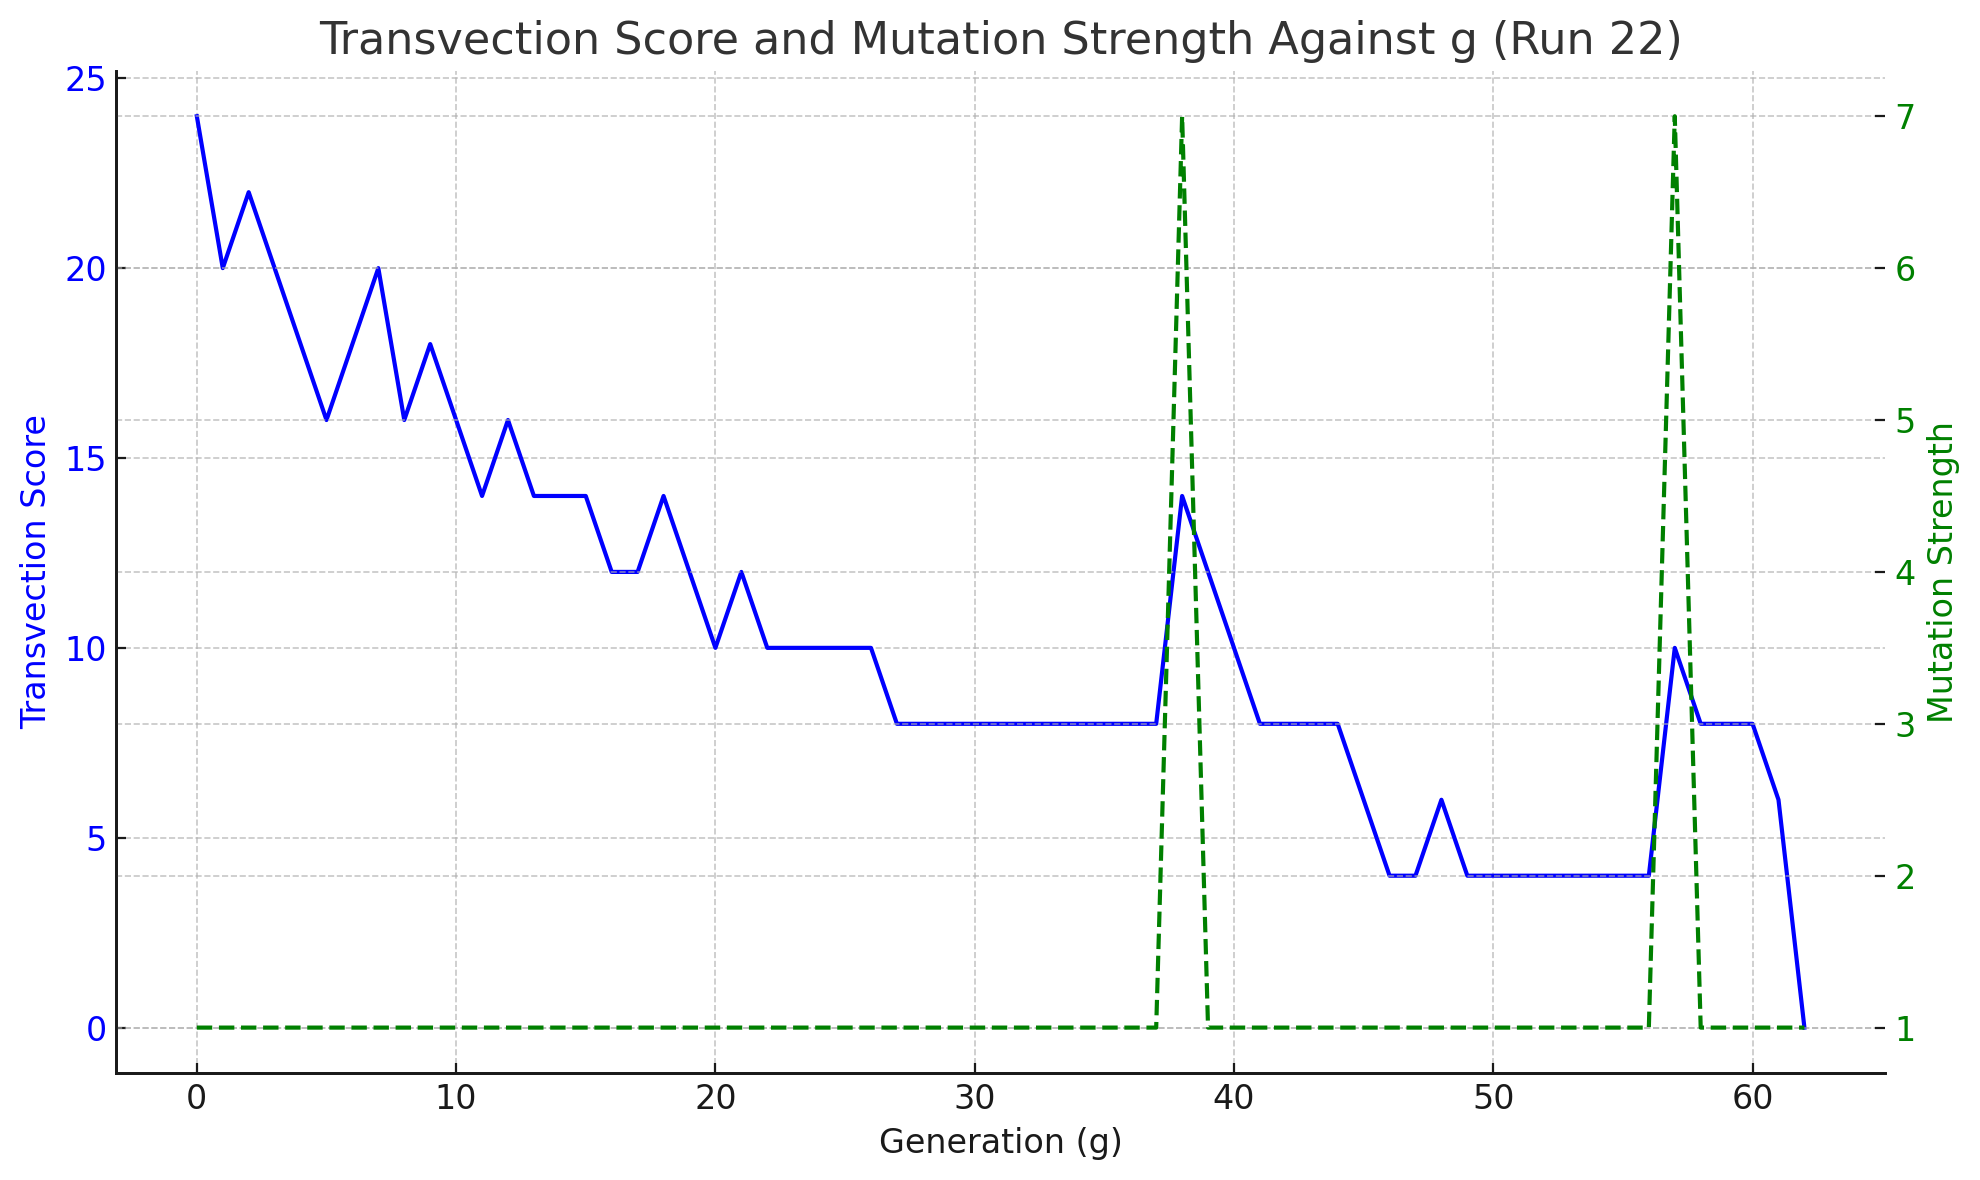
\includegraphics[width=1\linewidth]{Logos/output-4.png}
    \caption{Plot showing the total number of transvections per generation overlapped with the mutation strength across each generation on a single run of the [[7,1,3]] code to find lofical \(H\).}
    \label{fig: Adaptive Mutation tracker}
\end{figure}

Through empirical testing on the \([[5,1,3]]\) and \([[7,1,3]]\) codes, we found that strong mutation scales naturally with the number of qubits \(n\). Specifically, setting the strong mutation strength equal to \(n\) (i.e., 5 and 7 mutations respectively for the 5- and 7-qubit codes) yielded consistently good performance. In Figure \ref{fig: Adaptive Mutation tracker} we see how the transvection score evolves over generations alongside changes in mutation strength. The blue line represents the transvection score, which generally decreases as the algorithm progresses, indicating improved solutions. The green dashed line tracks the mutation strength, which increases adaptively when the score plateaus, signalling stagnation in the search process. Notably, spikes in mutation strength occur around generations 38 and 57, triggering a subsequent drop in transvection score shortly after. This illustrates the effectiveness of the adaptive mutation mechanism in helping the algorithm escape local minima and resume meaningful progress.

The experiments provided above, along with many more fine-tuning experiments, significantly contributed to the final model used to obtain the results, ensuring that the algorithm is well-calibrated for discovering low-transvection logical Clifford implementations across a range of stabiliser codes. These tests not only validated the effectiveness of individual parameter choices but also demonstrated their interplay in achieving robust, high-performance optimisation. The resulting configuration strikes a practical balance between search efficiency, solution quality, and scalability, making it suitable for use on a broad class of codes with varying sizes and structural properties.

\section{Rejected Approaches and Design Trade-offs}

\subsection{Evolutionary vs Greedy}
In this section, we briefly discuss alternative algorithmic approaches that were explored during development but ultimately deemed unsuitable for this task. While the backbone of the final implementation is an evolutionary search algorithm, one alternative we investigated was a greedy search strategy. In this approach, rather than sampling a fraction of possible single mutations per individual (as done in the evolutionary method), the algorithm exhaustively evaluates all possible single mutations and selects the best one at each step, proceeding iteratively in this greedy manner.

This method demonstrated promising results on smaller codes, such as the \([[5,1,3]]\) stabiliser code, especially when combined with enhancements like simulated annealing to introduce some stochasticity. In those cases, success rates were comparable to those achieved by the evolutionary algorithm. However, the greedy approach came with several significant drawbacks.

\begin{figure}[h]
    \centering
    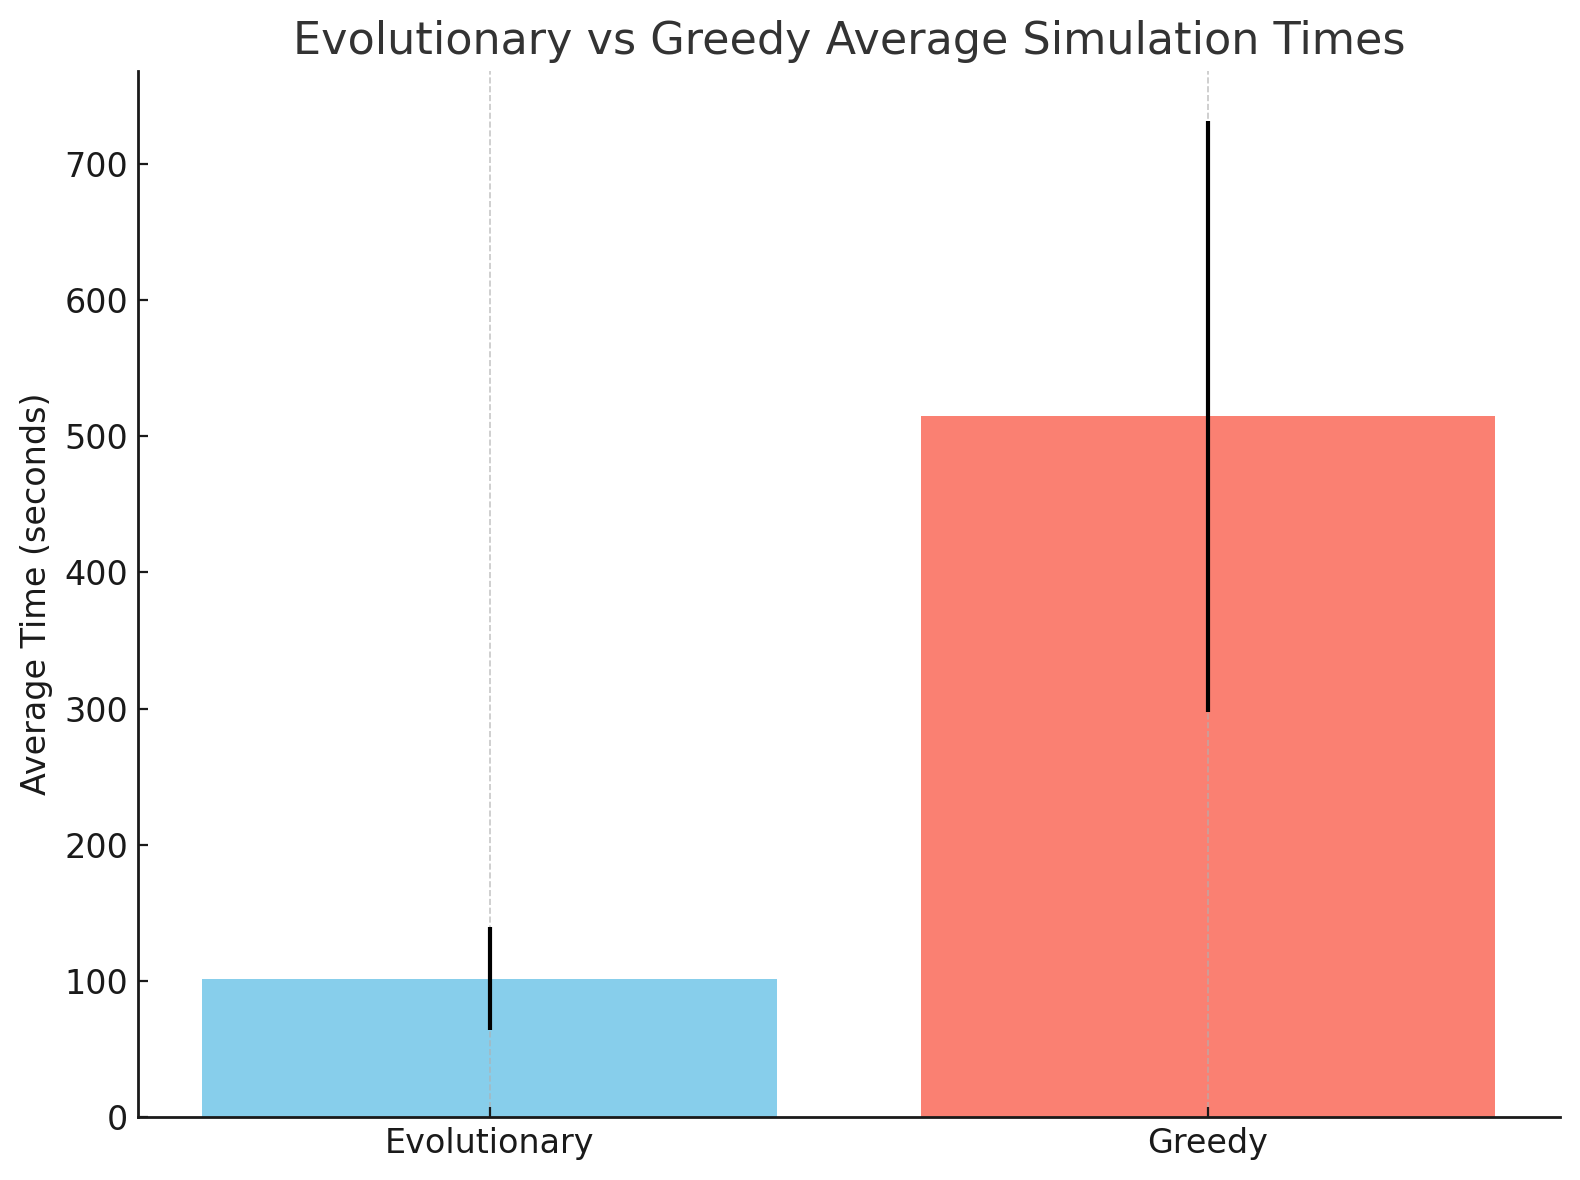
\includegraphics[width=1\linewidth]{Logos/output-5.png}
    \caption{Average simulation times on the \([[5,1,3]]\) code to find logical \(H\) for a standard Evolution and standard Greedy search algorithm. Number of runs = 36.}
    \label{fig:Evo vs Greedy simulation times}
\end{figure}

The most significant issue encountered was computational cost. Figure \ref{fig:Evo vs Greedy simulation times} compares the average execution times of the standard evolutionary algorithm and the greedy search algorithm. It is evident that the greedy approach is considerably slower, with an average runtime of \(515\) seconds per run, compared to just \(102\) seconds for the evolutionary algorithm. This discrepancy arises from the fundamental difference in how the two algorithms explore the mutation space. The evolutionary algorithm evaluates only a fraction, specifically \(1/(n-1)\), of the total mutation space per generation, the greedy approach examines the full set. This leads to an approximate runtime increase by a factor of \(n-1\), which becomes particularly prohibitive as the number of qubits grows. Moreover, the greedy method exhibited poor scalability. For larger codes, the mutation space becomes more rugged and populated with local minima, and the greedy approach by its very nature, lacks the exploration capabilities necessary to escape such traps. As a result, it often became stuck in suboptimal regions of the search space.

These limitations, both in terms of efficiency and robustness, ultimately led us to favour the evolutionary strategy, which strikes a more effective balance between exploration and exploitation and scales more gracefully with increasing code complexity.

\subsection{Dynamic Parameters}
Parameters such as the elite fraction, tournament size, and binary adaptive mutation strength were also considered in dynamic forms, meaning they would vary across generations during a single run, rather than remaining fixed. The motivation behind this approach was to better align the algorithm's behaviour with the demands of different phases of the search: for instance, using more exploration in early stages and gradually shifting toward exploitation in later ones.

However, our initial experiments with dynamic parameter schedules, conducted on the \([[5,1,3]]\) and \([[7,1,3]]\) codes, revealed mixed results. In most cases, the success rate either matched or fell slightly below that of the static configuration used in the final model. This may be partially attributed to the limited scope of codes tested; with only two small codes considered, it is difficult to draw definitive conclusions about the broader potential of dynamic parameters across more complex scenarios.

Another factor that may have influenced the outcome is the lack of optimisation in how the parameters changed over time for example, the rate at which elite fraction or mutation strength increased or decreased may not have been well-suited to the landscape of the optimisation problem. Without a principled or adaptive schedule, dynamic tuning can introduce instability or prevent the algorithm from settling into a productive search regime.

That said, this line of investigation remains promising, particularly for larger codes where the search dynamics may benefit more from stage-dependent behaviour. Future work could explore more data-driven or feedback-based scheduling of dynamic parameters, possibly leveraging online performance indicators such as population diversity or convergence rate to guide the adjustment process. 
%%%%%%%%%%%%%%%%%%%%%%%%%%%%%%%%%%%%%%%%%%%%%%%%%%%%%%%%%%%%%%%%%%%%%%%%%%%%%%%%
\chapter{Results and Analysis} \label{Chap4}

\section{Final Model}

\subsection{Success rate on Baseline codes}
The final model described in the methods section uses the evolutionary search algorithm as the main structure with implementations of elitism, tournaments selection and adaptive mutation rates. Through extensive testing on smaller codes namely the \([[5,1,3]]\) and \([[7,1,3]]\) codes we were able to fine tune parameters that scale moderately well with larger code sizes. In Figure \ref{fig:Final model success rate} below, we show the average success rate of the search algorithm at finding the minimum 2-qubit transvection implementations of the logical H and S operators on the \([[5,1,3]]\) and \([[7,1,3]]\) codes.

\begin{figure}[H]
    \centering
    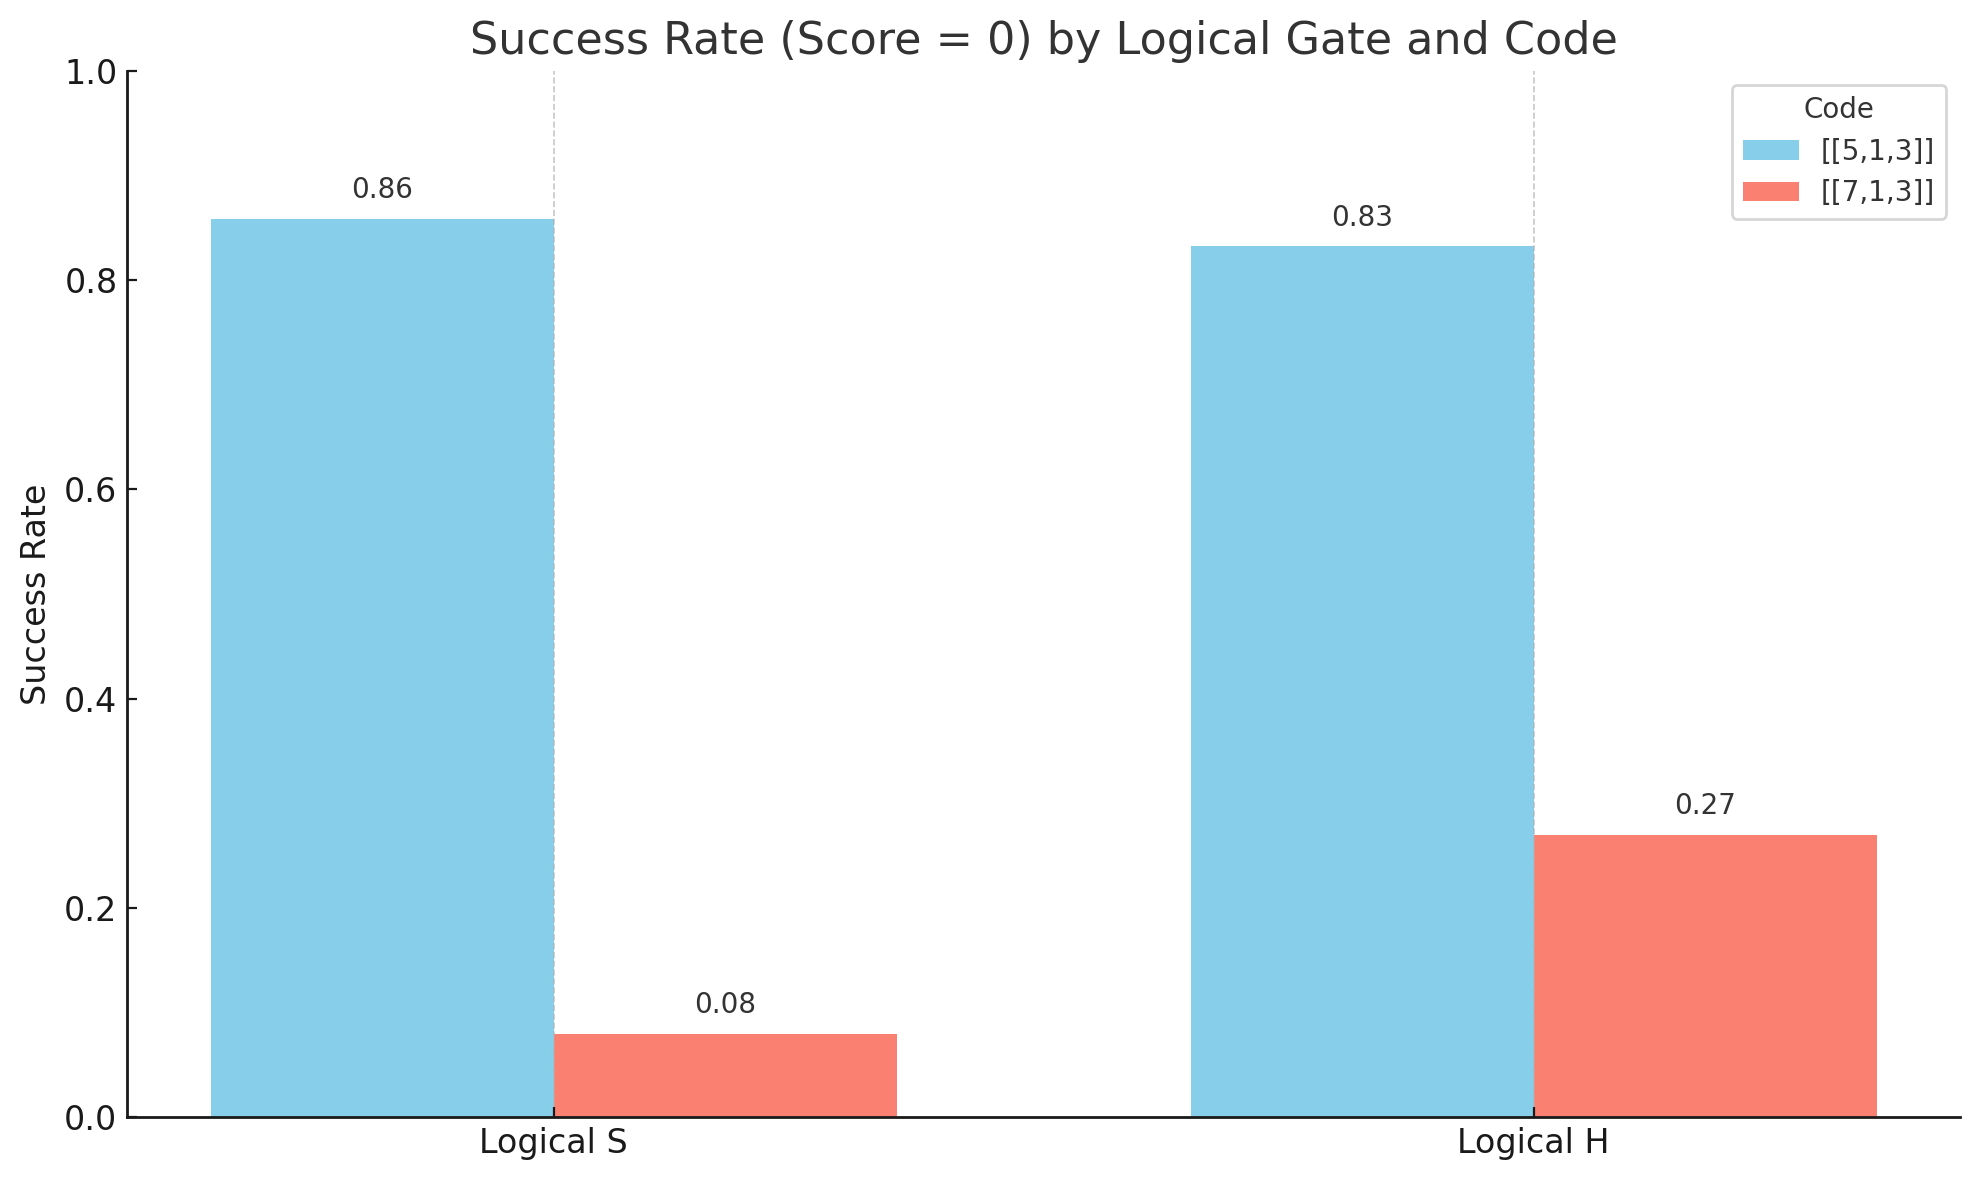
\includegraphics[width=1\linewidth]{Logos/output-6.png}
    \caption{Individual success rate of populations in the search algorithm for logical \(S\) and \(H\) in the [[5,1,3]] and [[7,1,3]] codes. number of runs: \((S,5)=500\), \((S,7)=88\), \((S,5)=1000\), \((S,5)=100\).}
    \label{fig:Final model success rate}
\end{figure}

Figure \ref{fig:Final model success rate} clearly illustrates the sharp decline in success rate when transitioning from the [[5,1,3]] code to the [[7,1,3]] code. This dramatic drop aligns with expectations when considering the exponential growth in search space. According to Equation \ref{eq:number of possible logical cliffords}, the [[5,1,3]] code yields a search space of approximately 5.28 billion possible implementations, whereas the [[7,1,3]] code expands this to an overwhelming \(1.73\times 10^{20}\), a difference of over 32.7 billion times. Given this massive increase, a corresponding decrease in the success rate of individual runs is anticipated.

In larger search spaces, not only is it harder to locate optimal solutions, but the likelihood of encountering numerous local minima also increases. Evidence of this can be found in Table \ref{tab:frequancy table of scores}, which shows that for the [[5,1,3]] code, the algorithm frequently converges to suboptimal scores of 2 and 4. This suggests the presence of at least two dominant local minima. In the case of the [[7,1,3]] code, the distribution of scores implies the presence of seven or more local minima, assuming these plateaus result from the algorithm becoming trapped, rather than from slow convergence. 

\begin{table}[h!]
\centering
\caption{Frequency of Scores (excluding 0) for logical \(H\)}
\label{tab:frequancy table of scores}
\begin{tabular}{ccc}
\toprule
\textbf{Score} & \textbf{[[5,1,3]]} & \textbf{[[7,1,3]]} \\
\midrule
2 & 96 & 6 \\
4 & 72 & 10 \\
6 & 0 & 15 \\
8 & 0 & 22 \\
10 & 0 & 16 \\
12 & 0 & 3 \\
14 & 0 & 1 \\
\bottomrule
\end{tabular}
\end{table}

\subsection{Model Execution times}
One last point to mention is the code runtime. For the [[5,1,3]] code we achieved a relatively short average execution time of \(135\pm 70\) seconds and the for the [[7,1,3]] this average time was \(4300\pm 600\) seconds. Similarly to before the this increase is expected as the search space increases drastically from [[5,1,1]] to [[7,1,3]]. A point to note is that the average runtime is approximately halved when the algorithm is executed serially rather than in parallel. This somewhat counterintuitive result is likely due to the behavior of Python's Just-In-Time (JIT) compiler, which may not optimize as effectively when using multiprocessing with a pool of worker processes. Despite this, running the algorithm in parallel remains the preferred approach. Even with a modest setup of 8 CPU cores, parallel execution effectively doubles the throughput compared to the serial version, allowing for significantly more runs to be completed in the same amount of time.

\section{Exploring implementations of the Toric Code}

\begin{figure}[h]
    \centering
    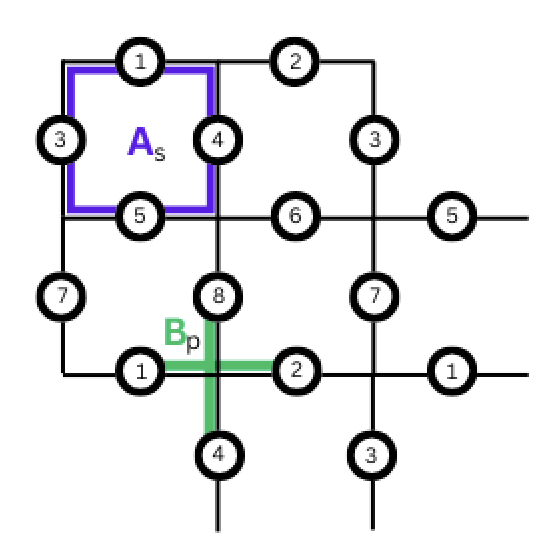
\includegraphics[width=0.5\linewidth]{Logos/Screenshot 2025-04-01 at 13.41.28.png}
    \caption{Repeating structure of the \([[8,2,2]]\) Toric code}
    \label{fig:[[8,2,2]] Toric code}
\end{figure}

The Toric code is a well known example of a topological stabiliser code (see Appendix \ref{Appendix C} that encodes quantum information into the global properties of a two-dimensional spin lattice. Its topological nature provides intrinsic protection against local errors, as logical qubits are stored non-locally across the lattice, making it particularly attractive for fault-tolerant quantum computing. Additionally, the Toric code's regular structure and compatibility with nearest-neighbour interactions make it well-suited for implementation on two-dimensional quantum hardware architectures. Here we have tested the algorithm on the \([[8,2,2]]\) Toric code to find low depth implementations logical \(S\), \(H\), \(CZ\), and \(CNOT\) (see Appendix \ref{Appendix D} for matrix representation of the Logical operators). These gates are not enough to perform universal computation however they do serve as a good showcase for the potential of our algorithm. Clifford gates are a foundational component of fault-tolerant quantum computing, especially in stabiliser code frameworks, and are often used in conjunction with magic state distillation to achieve universality. Efficient implementations of these logical operations are essential for reducing circuit depth, lowering error propagation, and improving overall computational fidelity.

\subsection{Logical S, H, CZ, and CNOT}
Using the algorithm, we were able to find an implementation of the logical \(\bar{S}\) gate consisting solely of single-qubit Clifford operations, meaning zero two-qubit transvections and, perhaps more surprisingly, no SWAP operations either. The resulting logical operator can be expressed as:

\begin{equation}
    \bar{S} = SIIIISII
\end{equation}

This compact form not only maintains full logical equivalence with the intended \(S\) gate on the encoded qubit, but also highlights how Clifford operations can sometimes be realised through entirely local, low-depth transformations when the structure of the code is properly leveraged. Such efficient representations are especially valuable in near-term devices, where circuit depth and entangling gates are limited by noise and hardware constraints.

For the logical H operator we also found a relatively low depth implementation consisting of a single 2-qubit transvection, some SWAPs and single-qubit Cifford layer;

Transvection \(T_v\):
\begin{equation}
    v_1 = Y_3X_7
\end{equation}

SWAPs:
\[
\begin{array}{cccccccc}
1 & 2 & 3 & 4 & 5 & 6 & 7 & 8 \\
\downarrow & \downarrow & \downarrow & \downarrow & \downarrow & \downarrow & \downarrow & \downarrow \\
2 & 6 & 3 & 4 & 1 & 5 & 7 & 8
\end{array}
\]

Single-qubit Cliffords:
\[
\begin{array}{ccccccccc}
qubit: & 1 & 2 & 3 & 4 & 5 & 6 & 7 & 8 \\
gate: & H & H & Y & HSH & H & H & Y & HSH
\end{array}
\]

For the logical CZ operator we can implement it as follows:

Transvections \(T_v\):
\begin{equation}
    v_1 = Y_1Z_4, \quad v_2=Y_2Z_4, \quad v_3=Z_3Y_5, \quad v_4=Z_3Y_6
\end{equation}

SWAPs:
\[
\begin{array}{cccccccc}
1 & 2 & 3 & 4 & 5 & 6 & 7 & 8 \\
\downarrow & \downarrow & \downarrow & \downarrow & \downarrow & \downarrow & \downarrow & \downarrow \\
1 & 2 & 3 & 8 & 5 & 6 & 7 & 4
\end{array}
\]

Single-qubit Cliffords:
\[
\begin{array}{ccccccccc}
qubit: & 1 & 2 & 3 & 4 & 5 & 6 & 7 & 8 \\
gate: & HS & HS & I & I & HS & HS & I & I
\end{array}
\]

And finally we can implement the CNOT as:

Transvections \(T_v\):
\begin{equation}
    v_1 = Z_3X_6, \quad v_2=X_1Z_8, \quad v_3=X_2Z_4, \quad v_4=Z_5X_7
\end{equation}

SWAPs:
\[
\begin{array}{cccccccc}
1 & 2 & 3 & 4 & 5 & 6 & 7 & 8 \\
\downarrow & \downarrow & \downarrow & \downarrow & \downarrow & \downarrow & \downarrow & \downarrow \\
6 & 1 & 4 & 3 & 2 & 7 & 8 & 5
\end{array}
\]

Single-qubit Cliffords:
\[
\begin{array}{ccccccccc}
qubit: & 1 & 2 & 3 & 4 & 5 & 6 & 7 & 8 \\
gate: & HSH & HSH & HS & S & HSH & HSH & HS & S
\end{array}
\]

Each implementation was verified to commute with the stabiliser group of the \([[8,2,2]] \) Toric code and to act on the logical subspace according to the expected transformation whilst preserving the stabiliser group. This ensures that all operators are indeed valid logical gates and preserve code space integrity.

It is important to note, however, that while the \(\bar{S}\) gate admits a particularly efficient implementation, not every logical Clifford operator will have a representation that avoids all two-qubit transvections. Moreover, the implementations of \(\bar{H},\space \bar{CZ}\) and \(\bar{CNOT}\) shown here may not represent the absolute optimal decompositions. For each of these gates, the algorithm was run between 24 and 32 times. Given that the 
\([[8,2,2]]\) Toric code has a significantly larger search space than smaller codes such as \([[5,1,3]]\) and \([[7,1,3]]\), it is likely that over 100 runs would be required to reliably discover the most efficient implementations.


%%%%%%%%%%%%%%%%%%%%%%%%%%%%%%%%%%%%%%%%%%%%%%%%%%%%%%%%%%%%%%%%%%%%%%%%%%%%%%%%
\chapter{Discussion} \label{Chap5}
The search algorithm we developed performs well for smaller codes, as demonstrated in the results section. However, its success rate, both for individual climbers and the overall system with multiple parallel populations, declines significantly as the code size increases. This drop in performance is likely due to the exponential growth of the search space with increasing code dimensions.

One straightforward solution to address the low success rate for larger codes is to increase the number of parallel populations. In our experiments, we were limited to a maximum of eight populations per run, constrained by the eight-core Apple M1 processor used for testing. This limitation, however, can be overcome by deploying the algorithm on a high-performance computing (HPC) cluster, such as UCL's Legion cluster, which offers access to over 7,500 CPU cores. Utilising such HPC resources would not only allow for a larger number of concurrent populations, thereby improving the algorithm's exploratory capacity, but would also significantly accelerate testing and parameter tuning.

In our case, testing was primarily conducted on the \([[5,1,3]]\) and \([[7,1,3]]\) quantum error-correcting codes, as they allowed for relatively faster data collection, although even these cases were time-consuming. Due to the limited number of code sizes tested and the resulting scarcity of performance data, it is difficult to conclusively assess the algorithm's robustness or scalability to much larger codes.

Beyond computational limitations, the algorithm itself still has room for improvement. One area worth exploring is the initial generation of the matrices \(U_C\) and \(U_A\). Currently, these matrices are initialised completely at random, which may lead some populations beginning their search in unfavorable regions of the search space, potentially getting stuck in local minima early on. Moreover, the lack of communication or coordination between initial populations means we cannot guarantee sufficient diversity at the start of each run. This can result in multiple populations redundantly exploring the same regions, thereby reducing overall efficiency.

Another promising direction for future enhancement is the integration of reinforcement learning (RL). RL strategies could be employed to dynamically control aspects of the search process, such as the type and location of mutations. Incorporating learning-based guidance could help the algorithm adapt more intelligently to the structure of the search space over time, improving both convergence speed and solution quality.

As demonstrated in the results section, we were able to find a constant-depth implementation of the logical \(S\) gate, along with relatively low-depth decompositions of the logical \(H\), \(CZ\), and \(CNOT\) operators. To the best of our knowledge, both the method used to discover these logical operators and the specific implementations themselves have not been previously documented in the literature. One notable related work is the recent paper Fault-Tolerant Constant-Depth Clifford Gates on Toric Codes by Alexandre Guernut and Christophe Vuillot \cite{guernut2024faulttolerantconstantdepthcliffordgates}, where the authors propose a framework for implementing the full Clifford group on 2D toric codes using fault-tolerant techniques such as fold-transversal gates, Dehn twists, and single-shot logical Pauli measurements.

While their approach is tailored specifically to topological codes like the toric code and relies on code-specific symmetries and geometric operations, the method presented in this paper is fundamentally different. Our algorithmic framework offers a more general and adaptable strategy that is not restricted to topological codes and can be applied to a wide variety of stabiliser codes. This broader applicability makes our approach particularly useful for synthesising logical Clifford gates in more diverse quantum error correction architectures.

%%%%%%%%%%%%%%%%%%%%%%%%%%%%%%%%%%%%%%%%%%%%%%%%%%%%%%%%%%%%%%%%%%%%%%%%%%%%%%%%
\chapter{Conclusion} \label{Chap6}
This thesis has presented an effective and scalable method for optimising logical Clifford operations in stabiliser quantum error-correcting codes through an evolutionary search algorithm. By minimising two-qubit transvections, the algorithm addresses one of the key practical limitations in fault-tolerant quantum computing, circuit depth and gate-induced error rates. Experimental validation across various stabiliser codes, including the Toric code, demonstrates the algorithm's ability to discover, low-depth implementations of Clifford gates such as \(S\), \(H\), \(CZ\), and \(CNOT\).

The findings show promising results, with success rates up to \(86\%\) on benchmark codes and significant simplifications in circuit design, especially for the logical S gate. Compared to existing techniques, the proposed method provides a more generalisable and efficient route to circuit optimisation, particularly for codes not previously studied in depth.

While the approach has shown strong performance on smaller codes, its full potential will be realised with greater computational resources and enhanced algorithmic strategies, such as machine learning-guided mutation. These advancements will not only enable application to larger codes but also pave the way for practical deployment in real-world quantum hardware. Ultimately, this research contributes a flexible and robust framework to support the ongoing pursuit of fault-tolerant, scalable quantum computation.

%%%%%%%%%%%%%%%%%%%%%%%%%%%%%%%%%%%%%%%%%%%%%%%%%%%%%%%%%%%%%%%%%%%%%%%%%%%%%%%%
\renewcommand{\bibname}{References}
\bibliographystyle{ieeetr}
%\bibliography{Bibliography.bib}
\bibliography{references.bib}
%%%%%%%%%%%%%%%%%%%%%%%%%%%%%%%%%%%%%%%%%%%%%%%%%%%%%%%%%%%%%%%%%%%%%%%%%%%%%%%%
% APPENDIX
\begin{appendices}
\chapter{Source Code} \label{Appendix A}
Source code for all of the methods implemented in Chap. \ref{Chap3} for the project can be found in the GitHub repository: \newline \url{link}. \newline \\
Project files can be found on Google Drive \url{link}

\chapter{Transvection decomposition} \label{Appendix B}
The Decomposition algorithm used is outlined as follows directly from the paper, Minimizing the Number of Two-qubit Gates in Clifford Circuits, by Kalle Volanto \cite{volanto2023minimizing}.

The algorithm begins by ensuring that the 2×2 block corresponding to the current qubit index on the matrix diagonal is invertible. If this is not the case, it searches for another row further down with an invertible block and swaps it into position. These swaps are considered cost-free due to the assumption that qubit relabeling is allowed.

Next, the algorithm eliminates any interfering entries in the current matrix column that originate from other rows. If there are multiple rows with non-zero, invertible sub-blocks in the same column, it constructs and applies appropriate two-qubit transvections to reduce redundancy. These operations simplify the structure by collapsing multiple interfering terms into a more manageable form.

After this, the algorithm scans for remaining non-zero entries in the current column, particularly those of rank one. For each such entry, it again constructs and applies a two-qubit transvection that zeroes out the unwanted term. This step ensures that the only non-zero contribution in the column comes from the diagonal block.

Finally, if the diagonal block is still not the identity matrix, the algorithm performs Gaussian elimination using one-qubit Clifford gates. These operations are applied to bring the block into standard form without incurring additional significant cost.

By the end of the iteration for each qubit, the symplectic matrix has been progressively simplified, and the sequence of operations required to implement the corresponding Clifford operator has been constructed. This method is particularly effective for small to medium-sized systems and offers a more direct alternative to traditional decomposition strategies, which often fragment the matrix into multiple subcomponents and lead to inefficient gate usage.

The algorithm below was directly taken from paper \cite{volanto2023minimizing} and displays the steps mentioned above in pseudo code.

\begin{algorithm}
\caption{Two-Qubit Transvection Decomposition Algorithm}
\label{alg:two_qubit_transvection}
\begin{algorithmic}[1]
\Require Symplectic matrix $F \in \text{Sp}(n, \mathbb{F}_2)$
\Ensure Sequence of SWAP gates, two-qubit transvections, and one-qubit transvections implementing $F$
\State sequence $\gets$ [\ ]
\For{$i \gets 1$ to $n$}
    \If{$R_F(i,i)$ is not invertible}
        \State Find $k > i$ such that $R_F(k,k)$ is invertible
        \State $F \gets \text{SWAP}_{i,k} \cdot F$
        \State sequence $\gets$ [SWAP$_{i,k}$] $\cup$ sequence
    \EndIf
    \While{there exist $j, k \neq i$ with invertible $R_F(j,i)$ and $R_F(k,i)$}
        \State Choose $c = F_{n+k,i}$ and $d = F_{k,i}$
        \State Choose $a$ and $b$ such that $[a,b] R_F(j,i) + [c,d] R_F(k,i) = [1,0]$
        \State $v = [a e_j + c e_k, b e_j + d e_k]$
        \State $F \gets T_v \cdot F$
        \State sequence $\gets$ [T$_v$] $\cup$ sequence
    \EndWhile
    \For{$k \gets i+1$ to $n$}
        \If{$\text{rank}(R_F(k,i)) = 1$}
            \State Choose $a,b,c,d$ such that $[d,c]^T [a,b] R_F(i,i) = R_F(k,i)$
            \State $v = [a e_i + c e_k, b e_i + d e_k]$
            \State $F \gets T_v \cdot F$
            \State sequence $\gets$ [T$_v$] $\cup$ sequence
        \EndIf
    \EndFor
    \While{$R_F(i,i) \neq I_2$}
        \State Choose a one-qubit transvection $T_v$ to perform Gaussian elimination on $R_F(i,i)$
        \State $F \gets T_v \cdot F$
        \State sequence $\gets$ [T$_v$] $\cup$ sequence
    \EndWhile
\EndFor
\State \Return sequence
\end{algorithmic}
\end{algorithm}


\chapter{Toric Code} \label{Appendix C}
The Toric code is defined on a square lattice with qubits placed on the edges, and periodic boundary conditions applied to form a torus. The code is characterised by two types of stabiliser generators: star operators \(A_s\)  and plaquette operators \(B_p\) as shown in Figure \ref{fig:[[8,2,2]] Toric code}. Each star operator acts as a tensor product of Pauli \(X\) operators on the four edges incident to a vertex \cite{bombin2013introduction}, i.e.,

\begin{equation}
    A_s=\Pi_{i\in s}X_i,
\end{equation}

while each plaquette operator is a product of Pauli \(Z\) operators around a face (plaquette), i.e., 

\begin{equation}
    B_p=\Pi_{i\in p}Z_i.
\end{equation}

The stabilisers define a code space as the simultaneous +1 eigenspace of all \(A_s\) and \(B_p\), enforcing constraints that detect both bit-flip and phase-flip errors. Because the stabilisers are local and commute, the code can be measured and corrected using only nearest-neighbour interactions, making it particularly appealing for physical realisation on planar architectures.

What makes the Toric code particularly attractive is its topological nature: logical qubits are encoded non-locally via operators that span the non-contractible loops of the torus. This non-local encoding grants the code inherent resilience against local noise, as local errors cannot easily accumulate to form logical errors unless they span the entire code distance \cite{eczoo_toric}. As a result, the Toric code achieves a high degree of fault tolerance with relatively low-weight stabilisers and minimal overhead.

Furthermore, the geometric regularity of the lattice and the reliance solely on nearest-neighbour interactions make the Toric code a natural fit for implementation on two-dimensional quantum hardware. It serves as a foundational example in the study of topological quantum computation and has inspired numerous extensions, including surface codes and color codes, which further generalize its principles to more practical, boundary-limited architectures.

\chapter{Symplectic Logical Operator matrices for the Toric code} \label{Appendix D}
The following matrices are the symplectic representations of the logical Clifford operators discussed in \ref{Chap3}. These matrices can be decomposed into 2-qubit transvection, SWAPs, and single qubit Cliffords using the transDecomp function found in the source code.


\begin{equation}
\label{mat:Logical S}
\bar{S}=
    \begin{bmatrix}
    1 & 0 & 0 & 0 & 0 & 0 & 0 & 0 & 1 & 1 & 0 & 0 & 0 & 1 & 1 & 1 \\
    0 & 1 & 0 & 0 & 0 & 0 & 0 & 0 & 0 & 0 & 0 & 0 & 1 & 0 & 1 & 1 \\
    0 & 0 & 1 & 0 & 0 & 0 & 0 & 0 & 0 & 0 & 0 & 0 & 0 & 0 & 0 & 0 \\
    0 & 0 & 0 & 1 & 0 & 0 & 0 & 0 & 0 & 0 & 0 & 0 & 0 & 0 & 0 & 0 \\
    0 & 0 & 0 & 0 & 1 & 0 & 0 & 0 & 0 & 0 & 0 & 0 & 0 & 1 & 1 & 1 \\
    0 & 0 & 0 & 0 & 0 & 1 & 0 & 0 & 0 & 0 & 0 & 0 & 0 & 1 & 1 & 1 \\
    0 & 0 & 0 & 0 & 0 & 0 & 1 & 0 & 0 & 0 & 0 & 0 & 0 & 0 & 0 & 0 \\
    0 & 0 & 0 & 0 & 0 & 0 & 0 & 1 & 0 & 0 & 0 & 0 & 0 & 0 & 0 & 0 \\
    0 & 0 & 0 & 0 & 0 & 0 & 0 & 0 & 1 & 0 & 0 & 0 & 0 & 0 & 0 & 0 \\
    0 & 0 & 0 & 0 & 0 & 0 & 0 & 0 & 0 & 1 & 0 & 0 & 0 & 0 & 0 & 0 \\
    0 & 0 & 0 & 0 & 0 & 0 & 0 & 0 & 0 & 0 & 1 & 0 & 0 & 0 & 0 & 0 \\
    0 & 0 & 0 & 0 & 0 & 0 & 0 & 0 & 0 & 0 & 0 & 1 & 0 & 0 & 0 & 0 \\
    0 & 0 & 0 & 0 & 0 & 0 & 0 & 0 & 0 & 0 & 0 & 0 & 1 & 0 & 0 & 0 \\
    0 & 0 & 0 & 0 & 0 & 0 & 0 & 0 & 0 & 0 & 0 & 0 & 0 & 1 & 0 & 0 \\
    0 & 0 & 0 & 0 & 0 & 0 & 0 & 0 & 0 & 0 & 0 & 0 & 0 & 0 & 1 & 0 \\
    0 & 0 & 0 & 0 & 0 & 0 & 0 & 0 & 0 & 0 & 0 & 0 & 0 & 0 & 0 & 1
    \end{bmatrix}
\end{equation}

\begin{equation}
\label{mat:Logical H}
\bar{H}=
    \begin{bmatrix}
    0 & 0 & 0 & 0 & 0 & 0 & 1 & 1 & 0 & 0 & 0 & 0 & 1 & 0 & 0 & 0 \\
    0 & 0 & 1 & 0 & 1 & 1 & 1 & 0 & 1 & 0 & 1 & 1 & 0 & 0 & 1 & 1 \\
    0 & 0 & 1 & 0 & 1 & 1 & 1 & 1 & 0 & 0 & 0 & 0 & 0 & 0 & 1 & 1 \\
    0 & 0 & 0 & 1 & 1 & 1 & 1 & 1 & 0 & 0 & 0 & 0 & 0 & 0 & 1 & 1 \\
    0 & 0 & 0 & 0 & 0 & 0 & 1 & 1 & 0 & 0 & 0 & 0 & 0 & 1 & 0 & 0 \\
    0 & 0 & 1 & 0 & 1 & 1 & 1 & 0 & 0 & 1 & 1 & 1 & 0 & 0 & 1 & 1 \\
    0 & 0 & 0 & 0 & 0 & 0 & 1 & 0 & 0 & 0 & 0 & 0 & 0 & 0 & 0 & 0 \\
    0 & 0 & 0 & 0 & 0 & 0 & 0 & 1 & 0 & 0 & 0 & 0 & 0 & 0 & 0 & 0 \\
    0 & 0 & 0 & 0 & 1 & 0 & 0 & 0 & 0 & 0 & 0 & 0 & 0 & 0 & 0 & 0 \\
    1 & 0 & 0 & 0 & 0 & 0 & 0 & 0 & 0 & 0 & 0 & 0 & 0 & 0 & 0 & 0 \\
    0 & 0 & 1 & 1 & 1 & 1 & 1 & 0 & 0 & 0 & 0 & 1 & 0 & 0 & 0 & 0 \\
    0 & 0 & 0 & 1 & 1 & 1 & 0 & 0 & 0 & 0 & 0 & 1 & 0 & 0 & 0 & 0 \\
    0 & 0 & 0 & 0 & 0 & 1 & 0 & 0 & 0 & 0 & 0 & 0 & 0 & 0 & 0 & 0 \\
    0 & 1 & 0 & 0 & 0 & 0 & 0 & 0 & 0 & 0 & 0 & 0 & 0 & 0 & 0 & 0 \\
    0 & 0 & 0 & 1 & 0 & 0 & 0 & 0 & 0 & 0 & 1 & 1 & 0 & 0 & 1 & 0 \\
    0 & 0 & 0 & 0 & 0 & 0 & 0 & 1 & 0 & 0 & 0 & 0 & 0 & 0 & 0 & 1
    \end{bmatrix}
\end{equation}

\begin{equation}
\label{mat:Logical CZ}
\bar{CZ}=
    \begin{bmatrix}
    1 & 0 & 0 & 0 & 0 & 0 & 0 & 0 & 1 & 0 & 0 & 0 & 0 & 0 & 0 & 1 \\
    0 & 1 & 0 & 0 & 0 & 0 & 0 & 0 & 0 & 1 & 0 & 0 & 0 & 0 & 0 & 1 \\
    0 & 0 & 1 & 0 & 0 & 0 & 0 & 0 & 0 & 0 & 0 & 0 & 1 & 1 & 0 & 0 \\
    1 & 1 & 0 & 0 & 0 & 0 & 0 & 1 & 0 & 0 & 0 & 0 & 0 & 0 & 0 & 0 \\
    0 & 0 & 0 & 0 & 1 & 0 & 0 & 0 & 0 & 0 & 1 & 0 & 1 & 0 & 0 & 0 \\
    0 & 0 & 0 & 0 & 0 & 1 & 0 & 0 & 0 & 0 & 1 & 0 & 0 & 1 & 0 & 0 \\
    0 & 0 & 0 & 0 & 0 & 0 & 1 & 0 & 0 & 0 & 0 & 0 & 0 & 0 & 0 & 0 \\
    0 & 0 & 0 & 1 & 1 & 1 & 0 & 0 & 0 & 0 & 0 & 0 & 1 & 1 & 0 & 0 \\
    0 & 0 & 0 & 0 & 0 & 0 & 0 & 0 & 1 & 0 & 1 & 1 & 0 & 0 & 1 & 0 \\
    0 & 0 & 0 & 0 & 0 & 0 & 0 & 0 & 0 & 1 & 1 & 1 & 0 & 0 & 1 & 0 \\
    0 & 0 & 0 & 0 & 0 & 0 & 0 & 0 & 0 & 0 & 1 & 0 & 0 & 0 & 0 & 0 \\
    0 & 0 & 0 & 0 & 0 & 0 & 0 & 0 & 0 & 0 & 0 & 0 & 0 & 0 & 0 & 1 \\
    0 & 0 & 0 & 0 & 0 & 0 & 0 & 0 & 0 & 0 & 1 & 0 & 1 & 0 & 1 & 1 \\
    0 & 0 & 0 & 0 & 0 & 0 & 0 & 0 & 0 & 0 & 1 & 0 & 0 & 1 & 1 & 1 \\
    0 & 0 & 0 & 0 & 0 & 0 & 0 & 0 & 0 & 0 & 0 & 0 & 0 & 0 & 1 & 0 \\
    0 & 0 & 0 & 0 & 0 & 0 & 0 & 0 & 0 & 0 & 0 & 1 & 0 & 0 & 0 & 0
    \end{bmatrix}
\end{equation}

\begin{equation}
\label{mat:Logical CNOT}
\bar{CNOT}=
    \begin{bmatrix}
    0 & 1 & 0 & 1 & 1 & 1 & 0 & 1 & 0 & 0 & 0 & 0 & 0 & 0 & 0 & 0 \\
    0 & 0 & 0 & 0 & 1 & 0 & 0 & 0 & 0 & 0 & 0 & 0 & 0 & 0 & 0 & 0 \\
    1 & 0 & 0 & 1 & 1 & 1 & 0 & 0 & 0 & 0 & 0 & 0 & 0 & 0 & 0 & 0 \\
    0 & 0 & 1 & 0 & 0 & 1 & 0 & 0 & 0 & 0 & 0 & 0 & 0 & 0 & 0 & 0 \\
    0 & 0 & 0 & 0 & 0 & 1 & 0 & 0 & 0 & 0 & 0 & 0 & 0 & 0 & 0 & 0 \\
    1 & 0 & 0 & 0 & 0 & 0 & 0 & 0 & 0 & 0 & 0 & 0 & 0 & 0 & 0 & 0 \\
    0 & 0 & 0 & 0 & 0 & 1 & 0 & 1 & 0 & 0 & 0 & 0 & 0 & 0 & 0 & 0 \\
    0 & 1 & 0 & 1 & 1 & 1 & 1 & 1 & 0 & 0 & 0 & 0 & 0 & 0 & 0 & 0 \\
    0 & 0 & 0 & 0 & 0 & 0 & 1 & 0 & 0 & 1 & 1 & 1 & 0 & 0 & 0 & 1 \\
    0 & 0 & 1 & 0 & 1 & 1 & 0 & 0 & 0 & 0 & 1 & 0 & 1 & 0 & 1 & 1 \\
    0 & 0 & 0 & 0 & 0 & 0 & 0 & 0 & 0 & 0 & 0 & 1 & 0 & 1 & 1 & 1 \\
    0 & 0 & 1 & 0 & 1 & 1 & 0 & 0 & 0 & 0 & 1 & 0 & 0 & 0 & 0 & 0 \\
    0 & 0 & 0 & 0 & 0 & 0 & 0 & 0 & 0 & 0 & 0 & 0 & 0 & 0 & 0 & 1 \\
    0 & 0 & 0 & 0 & 0 & 0 & 0 & 0 & 1 & 0 & 1 & 0 & 0 & 1 & 0 & 0 \\
    0 & 0 & 0 & 0 & 0 & 0 & 0 & 0 & 0 & 0 & 0 & 0 & 0 & 1 & 1 & 0 \\
    0 & 0 & 0 & 0 & 0 & 0 & 1 & 0 & 0 & 0 & 0 & 0 & 0 & 0 & 1 & 0
    \end{bmatrix}
\end{equation}



\end{appendices}
%%%%%%%%%%%%%%%%%%%%%%%%%%%%%%%%%%%%%%%%%%%%%%%%%%%%%%%%%%%%%%%%%%%%%%%%%%%%%%%%
% GLOSSARY
\clearpage
\printglossaries

% INDEX?

\end{document}